%\documentclass{article} % opcje: robocza,man
\documentclass{mgragh} % opcje: robocza,man
\usepackage{float}
\usepackage[cp1250]{inputenc}  % opcja latin2 dla Linuxa lub cp1250 dla Windows
\usepackage[polish]{babel}
\usepackage[OT4]{fontenc}
\usepackage{polski}
%\usepackage{graphicx}
\usepackage[urlcolor=blue, colorlinks=true, bookmarks=true, bookmarksnumbered=true]{hyperref}

\usepackage{epsfig}


%%
%%
\makeindex

%\bibliographystyle{ddabbrv}
\bibliographystyle{bibtex}
%\nocite{*}

\begin{document}
%%
%%
%% ======== METRYCZKA PRACY ========
\title{Komponentowa architektura indukcyjnej bazy danych jako platformy uczenia
maszynowego}
\author{Nikodem Jura, Krzysztof Rajda}
\promotor{dr hab. in�. Marek Kisiel-Dorohinicki}
\nralbumu{11957}
\uczelniaNazwa{Akademia G�rniczo-Hutnicza}
\uczelniaImienia{im. Stanis�awa Staszica}
\wydzial{Elektroniki, Automatyki, Informatyki i Elektrotechniki}
\kierunek{Informatyka}
\specjalnosc{In�ynieria system�w informatycznych i baz danych}
\rok{2006}

%\maketitle
%%
\slowakluczowe{}

\keywords{a,b,c,d,e,f,g,h} 
%%
%%
%% ======== NASZE MAKRA ========
%%

%----------------- nasze definicje -----------------% 
\newtheorem{stw}{\indent Stwierdzenie}[chapter]
%------------------------------%
\newcommand{\id}[1]{\index{#1}}  
\newcommand{\wi}[1]{#1\index{#1}}  
\newcommand{\wwi}[1]{\emph{#1}\index{#1}}  
\newcommand{\mwi}[1]{\textbf{#1}\index{#1}}
\newcommand{\ii}[1]{\textit{#1}}
%\newcommand{}{}

%---------------------------------------------------%



%%
%% ======== SPIS TRE�CI ========
%%
\tableofcontents
%%
%% ======== STRESZCZENIE PRACY (POLSKIE) ========
\begin{streszczenie}
%%

%--------------------------------------------------------------------%

%%
\end{streszczenie}
%%
%% ======== G��WNA CZʌ� PRACY ========
%%
%% ==== WST�P ====
%%
\begin{wstep}
%%
\section{Wprowadzenie}
%\subsection{Machine learning}
%\subsection{Indukcyjne bazy danych}
%\subsection{Zastosowania}

Integracja technologii baz danych z nowoczesnymi metodami indukcyjnego
generowania wiedzy wydaje si� dawa� istotne korzy�ci w perspektywie
budowy system�w wspomaganie decyzji. Systemy nazywane czasem
indukcyjnymi bazami danych potrafi� odpowiedzie� nie tylko na pytania,
dla kt�rych odpowied� znajduje si� w bazie danych, ale r�wnie� na
pytania, kt�re wymagaj� zsyntetyzowania i zastosowania wiarygodnej
wiedzy, wygenerowanej przez indukcyjne wnioskowanie z fakt�w z bazy
danych i wcze�niejszej wiedzy.  Indukcyjne bazy danych mog� by�
postrzegane jako naturalny krok w rozwoju system�w bazodanowych \cite{bib3}.

\begin{figure}[ht]
    \centering
        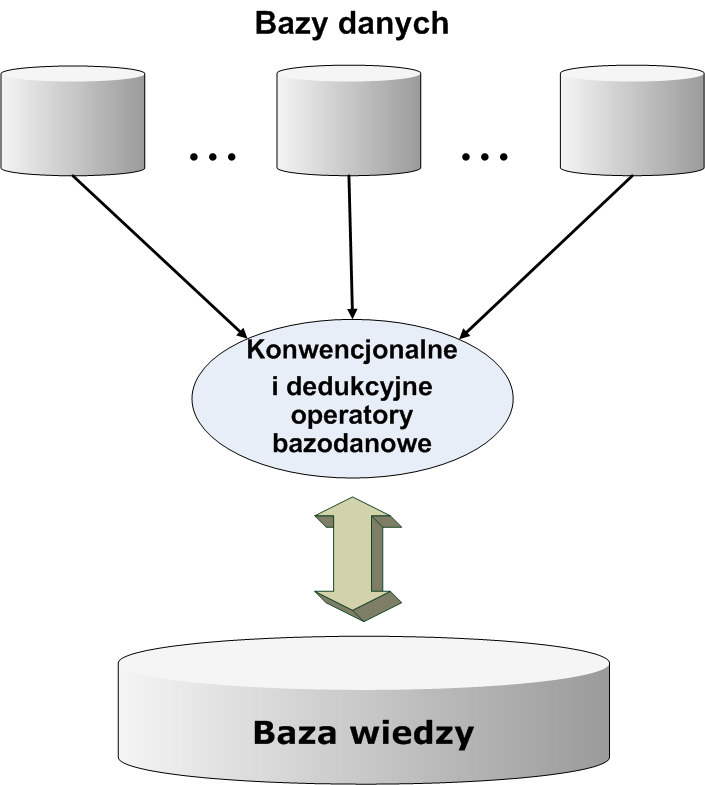
\includegraphics[width=0.70\textwidth]{img/knowledge_mining.png}
    \caption{Indukcyjne bazdy danych}
    \label{fig:architecture}
\end{figure}

\bigskip
W pracy przedstawiona zostanie architektura i wybrane aspekty
implementacji platformy \emph{Salomon}, jak r�wnie� zaprezentowane
zostan� mo�liwo�ci jego wykorzystania na przyk�adzie wybranych
algorytm�w pozyskiwania wiedzy z danych.

%\newpage
%%
\end{wstep}
%%
%% ==== ROZDZIA� 1 ====
%%
%% A tutaj tak dla przyk�adu jest \part
\part{Wprowadzenie}

%%
\chapter{Uczenie maszynowe}
%Cichosz (35-36)
\section{Algorytmy ucz�ce si�}

Pr�by opracowania algorytm�w ucz�cych si� nie wynikaj� z ch�ci wyeliminowania
projektant�w z proces�w analizy i projektowania system�w komputerowych, a wi�c
klasycznych zagadnie� in�ynierii oprogramowania. Nie mog� one bowiem by�
alternatyw� dla tradycyjnych metodologii tworzenia oprogramowania. Cele, jakie
stawiaj� sobie tw�rcy algorytm�w ucz�cych si� wynikaj� ze z�o�ono�ci niekt�rych
zagadnie� algorytmicznych -- pr�buj� oni w�a�nie za ich pomoc� opisa� te
problemy, dla kt�rych opracowanie poprawnych i pe�nych algorytm�w klasycznych
jest bardzo trudne lub wr�cz niemo�liwe.

Program ucz�cy mo�na wyobrazi� sobie jako abstrakcyjny, ,,parametryzowalny''
algorytm wykonania zadania. Proces uczenia polega na dobraniu, na podstawie
historycznych warto�ci tych ,,parametr�w'', takich warto�ci, by rozwi�zanie
spe�nia�o za�o�enia projektanta. 

,,Parametry'' te mo�na traktowa� jako pewnego rodzaju \emph{wiedz�}.
Nie s� one podawane do algorytmu w spos�b bezpo�redni (a je�li nawet s� podawane
ich pocz�tkowe warto�ci, to s� one najcz�ciej dalekie od oczekiwanych), ale
odkrywane s� przez sam algorytm podczas procesu uczenia si�.
Z tego te� powodu s� one traktowane jako wiedza niepewna i mog�ca wymaga� weryfikacji.	

Wiedza ta mo�e okre�la� zar�wno sekwencje operacji, kt�re program ma wykona�
podczas rozwi�zywania danego problemu, jak i wyb�r spo�r�d r�nych wariant�w
mo�liwych do podj�cia w danym momenecie decyzji.

Wiedza, kt�ra okre�la strategie osi�gania cel�w nazywana jest
\emph{proceduraln�}, natomiast taka, kt�ra opisuje obiekty i zwi�zki mi�dzy nimi
-- \emph{deklaratywn�}.

Algorytmy pozyskiwania i doskonalenia zdobytej wiedzy nazywane s�
\emph{algorytmami uczenia maszynowego}. 

% Cichosz 40
%\subsection{Zastosowanie algorytm�w ucz�cych}

Zastosowanie algorytm�w uczenia maszynowego jest bardzo szerokie.
Zdarza si�, �e ich wykorzystanie do rozwi�zania niekt�rych problem�w
mo�e by� tak�e podyktowane czynnikami ekonomicznymi -- czasem bardziej op�aca
si� zastosowa� algorytmy ucz�ce si�, ni� traci� czas na opracowywanie 
skomplikowanych algorytm�w klasycznych, kt�re i tak w pewnych przypadkach mog�
dzia�a� niepoprawnie.

Dla naprawd� du�ych i z�o�onych problem�w trudne jest opracowanie pe�nych i~poprawnych 
algorytm�w je rozwi�zuj�cych. Z takimi przypadkami mamy do czynienia
np. w zagadnieniach dotycz�cych realnie dzia�aj�cych system�w, w kt�rych trzeba
liczy� si� z du�� dynamik� i nieprzewidywalno�ci� �rodowiska, w kt�rym dzia�a program.
Uzyskanie poprawnie dzia�aj�cych algorytm�w pracuj�cych w takich systemach mo�e
okaza� si� bardzo kosztowne: albo ze wzgl�du na czas i �rodki potrzebne do ich
opracowania, albo ze wzgl�du na zasoby u�ywane podczas ich pracy. Zdarza si�
tak�e, ze opracowanie zadowalaj�cych algorytm�w jest wr�cz niemo�liwe.
Wynika to z tego, �e �rodowiska w kt�rych cz�sto musz� dzia�a� takie algorytmy
s� trudne do opisania -- brakuje dla nich modeli teoretycznych, lub te�
uproszczenia, kt�re musia�y zosta� w nich przyj�te, by wog�le mo�liwe by�o
opisanie danego �rodowiska nie pozwalaj� na uzyskanie wystarczaj�co dok�adnie
dzia�aj�cych algorytm�w.

W wielu zastosowaniach systemy informatyczne powinny dzia�a� mo�liwe
autonomicznie i wymaga� znikomej ingerencji ze strony cz�owieka. Przyk�adami
takich system�w mog� by� systemy kontroli poszczeg�lnych instalacji w
nowoczesnych biurowcach, systemy sterowania robotami przemys�owymi czy pojazdami
bezza�ogowymi. Wymagany stopie� autonomii tych system�w jest niemo�liwy do
uzyskania bez wyposa�enia ich w mo�liwo�� adaptacji, czyli przystosowania si� do
zmieniaj�cych si� warunk�w. Systemy posiadaj�ce zdolno�� adaptacji mog� by�
u�ywane w nieprzewidywalnym �rodowisku lub wielu podobnych �rodowiskach.

Jednym z najwa�niejszych zastosowaniem algorytm�w ucz�cych jest nowoczesna
analiza danych, tzw. \emph{data mining}.
Wsp�czesne zbiory danych, kt�re musz� by� poddawane analizie pochodz� np.
z d�ugotrwa�ych pomiar�w i eksperyment�w naukowych. Zawieraj� ogromne ilo�ci
danych, co powoduje, ze nie mog� one by� analizowane w inny spos�b, ni�
automatycznie. Do ich filtrowania i wyszukiwania zale�no�ci mi�dzy nimi
wykorzystuje si� specjalnie opracowane algorytmy, kt�re potrafi� nie tylko
przetwarza� dane aktualne, ale tak�e wnioskowa� na podstawie danych historycznych,
przechowywanych w ogromnych bazach danych, zwanych \emph{hurtowniami danych}.

%Troche przykladow
\subsection{Metody reprezentacji wiedzy}

% Cichosz 41-42
Wiedza z punktu widzenia algorytm�w ucz�cych mo�e by� przechowywana na r�ne
sposoby -- opracowano w tym celu wiele efektywnych struktur danych,
pozwalaj�cych na jej �atwe zapisanie i przetwarzanie.
Z regu�y jednak dziedzina, w jakiej ma byc wykorzystany algorytm ucz�cy,
determinuje, lub w najlepszym przypadku zaw�a, ilo�� mo�liwych reprezentacji
wiedzy, z kt�rych ka�da ma swoje dobre strony jak i ograniczenia.
Do podstawowych metod reprezentacji wiedzy nale�� drzewa decyzyjne, formu�y
logiki predykat�w, wykorzystuje si� tak�e rozk�ady prawdopodobie�stwa oraz
automaty sko�czone.

Jednym z podzia��w metod reprezentacji wiedzy jest rozr�nienie mi�dzy metodami
\emph{symbolicznymi} i \emph{subsymbolicznymi}.
Metody symboliczne do reprezentacji wiedzy stosuj� struktury przechowywuj�ce
informacje o chartakterze symbolicznym, czyli pewne napisy, kt�re mog� by� w
pewien spos�b interpretowane. Napisy te najcz�ciej maj� form� czyteln� dla
cz�owieka i mog� by� przez niego przegl�dane i poddawane analizie i
interpretacji. 
Metody drugiej z kategorii przechowuj� informacje w formie trudnej do
interpretacji przez cz�owieka. Poszczeg�lne dane analizowane
pojedynczo nie nios� �adnej sensownej informacji, gdy� cz�sto s� to ci�gi liczb
lub dane binarne. Dopiero odpowiednio po��czone ze sob� dane poddane
przetwarzaniu reprezentuj� pewn� wiedz�.

Nie zawsze metoda u�yta do reprezentacji wiedzy dla okre�lonych zastosowa� jest
jedynym mo�liwym sposobem jej przedstawienia, jednak rzadko zdarza si�, by wyb�r
metody by� szeroki. Wynika to z tego, �e spos�b, w jaki wiedza mo�e by� u�yta
zale�y g��wnie od wyboru metody oraz celu, czyli zadania, kt�re ma by� wykonane
przez algorytm ucz�cy.

Do najpowszechniejszych zada�, kt�re stawia si� przed algorytmami ucz�cymi
nale�� klasyfikacja i aproksymacja. Klasyfikacja ma na celu ustalenie
przynale�no�ci danych obiekt�w do okre�lonych kategorii, natomiast aproksymacja
polega na odzworowaniu obiekt�w na zbi�r liczb rzeczywistych.

Algorytmy ucz�ce mog� tak�e by� wykorzystane do innych zastosowa�, jak np.
sekwencyjne podejmowanie decyzji, czy te� modelowanie z�o�onych �rodowisk, dla
kt�rych opracowanie klasycznych modeli jest trudne, lub nawet niemo�liwe.
Znajduj� one tak�e zastosowanie jako narz�dzia wspomagaj�ce cz�owieka w
przetwarzaniu du�ej ilo�ci informacji -- mog� one przedstawia� wiedz� uzyskan� z
analizy du�ej ilo�ci danych w bardziej czytelnej dla cz�owieka formie.

% Cichosz 43-44
\subsection{Podzia� algorytm�w ucz�cych}

Jednym z najbardziej podstawowych kryteri�w podzia�u algorytm�w ucz�cych si� jest
ich podzia� na  \emph{uczenie si� z nadzorem} i \emph{bez nadzoru}.

W przypadku uczenia z nadzorem (czasami nazywanego tak�e \emph{uczeniem z
nauczycielem}) wiedza uzyskiwana w czasie dzia�ania algorytmu ucz�cego jest
weryfikowana -- algorytm dla okre�lonych danych wej�ciowych otrzymuje tak�e
oczekiwane informacje wyj�ciowe, zwane \emph{informacj� trenuj�c�}.
Zadaniem procesu uczenia si� jest takie dobranie parametr�w algorytmu, aby dla
okre�lonych danych wej�ciowych otrzyma� dane wyj�ciowe mo�liwie zbli�one do
wzorcowych.

W procesie uczenia bez nadzoru nie jest dost�pna informacja trenuj�ca. Podawane
s� jedynie dane wej�ciowe i jedynie na ich podstawie algorytm ma si�
,,nauczy�'' prawid�owo je interpretowa�. Z takimi przypadkami mamy do czynienia
g��wnie w algorytmach grupuj�cych obiekty, gdzie nie s� znane kryteria, wed�ug
kt�rych obiekty maj� zosta� pogrupowane. Czasem m�wi si�, �e takie algorytmy
maj� wbudowanego nauczyciela, jako �e weryfikacja uzyskiwanej wiedzy jest
integraln� cz�ci� algorytmu.

Uczenie z nauczycielem i bez nadzoru to najbardziej popularne grupy algorytm�w,
jednak wyr�nia si� tak�e inne. Podobn� do uczenia z nadzorem grup� algorytm�w
s� metody \emph{uczenia na podstawie zapyta�}. W takim przypadku informacja
trenuj�ca co prawda pochodzi od nauczyciela, lecz stanowi jedynie odpowied� na
zadane przez ucznia pytanie. W odr�nieniu od uczenia pod nadzorem, nauczyciel
nie podaje przyk�ad�w danych wej�ciowych i oczekiwanych odpowiedzi, a jedynie
odpowiada na jawne pytanie ucznia.

Mo�na tak�e wyr�ni� metod� \emph{uczenia przez eksperymentowanie}. Mamy z ni�
do czynienia, gdy algorytm gromadzi wiedz� poprzez wykonywanie eksperyment�w ze
�rodowiskiem, w kt�rym dzia�a. Polega to na wykonywaniu pewnych dzia�a�, a
nast�pnie obserwowaniu ich konsekwencji i wp�ywu, jakie maj� one na �rodowisko.

Zbli�on� to uczenia przez eksperymentowanie metod� jest \emph{uczenie ze
wzmocnieniem}. Podobnie jak poprzednia metoda opiera si� ono na
eksperymentowaniu, jednak wykorzystuje dodatkowo pewn� informacj� trenuj�c�,
pozwalaj�c� na ocen� uzyskanej wiedzy. W tym przypadku informacja ta nie 
ma charakteru instrukta�owego, ale pozwala na otrzymanej warto�ciowanie wiedzy
poprzez przypisanie jej liczbowych wsp�czynnik�w zwanych \emph{wzmocnieniami}.
Pozwala to na ocen� dotychczasowego przebiegu procesu uczenia si� i dobieranie
jego parametr�w tak, by uzyskiwana by�a wiedza zbli�ona do tej z najwy�szymi wsp�czynnikami. 

\subsection{Metody uczenia si�}

% Cichosz 44
Informacja trenuj�ca stanowi dla algorytmu ucz�cego si� podstaw�, kt�r�
wykrzystuje do nabywania nowej wiedzy lub do udoskonalenia ju� posiadanej.
Reprezentacja tej wiedzy oraz spos�b jej wykorzystania najcze�ciej
podporz�dkowany jest zadaniu, do realizacji kt�rego ma zosta� u�yta.
Mechanizm odkrywania nowej lub ulepszania ju� posiadanej wiedzy z regu�y mocno
zale�y od sposobu jej reprezentacji oraz postaci informacji trenuj�cej.

Z regu�y do realizacji konkretnego mechanizmu zdobywania wiedzy mog� by� u�yte
r�norodne algorytmy.
Najbardziej popularn� metod� uczenia si� jest \emph{indukcja}. Polega ona na
wnioskowaniu na podstawie posiadanej, konkretnej, informacji trenuj�cej. Ma ona
na celu celu uzyskania wiedzy og�lnej za pomoc� uog�lnienia informacji
trenuj�cej na pozosta�e przypadki.

Opr�cz metod indukcyjnych, wyr�nia si� tak�e mechanizmy \emph{uczenia
nieindukcyjnego}. Metody te maja na celu nie tyle wnioskowanie, ile raczej 
wyja�nianie -- informacja trenuj�ca nie jest uog�lniania, lecz wykorzystywana
jest do konkretyzacji ju� zdobytej przez algorytm ucz�cy si� wiedzy.
% Add reference here - uczenie ze wzmocnieniem
Do metod tych zalicza si� tak�e stosowane przy uczeniu ze wzmocnieniem
warto�ciowanie zdobytej wiedzy pozwalaj�ce na lepsze wyselekcjonowanie
po�ytecznej wiedzy.

%Cichosz 45 - glowne dzialy uczenia maszynowego
\subsection{G��wne nurty uczenia maszynowego}

Badania nad r�nymi systemami ucz�cymi doprowadzi�y to powstania nowej dziedziny
naukowej -- \emph{uczenia maszynowego}. Dziedzina ta mo�e by� traktowana jako
ga��� sztucznej inteligencji, czy szerzej -- informatyki.
W zg��bianie zagadnie� uczenia maszynowego zaanga�owani s� nie tylko
informatycy, co wydaje si� naturalne, ale tak�e przedstawiciele innych dziedzin
takich jak matematyka, a nawet psychologia, czy biologia.

%za Cichoszem
Wydziela si� 3 g��wne nurty, w kt�rym zmierzaj� prace badawcze w dziedzinie
uczenia maszynowego -- nurt \emph{teoretyczny}, \emph{biologiczny} i \emph{systemowy}.

Badacze zajmuj�cy si� nurtem teoretycznym stawiaj� sobie za cel przede
wszystkim rozwijanie podstaw teoretycznych, na kt�rych ma opiera� si� ca�a
dziedzina. Staraj� si� oni nazwa� i usystematyzowa� poj�cia zwi�zane z t�
dziedzin� i d��� do utworzenia s�ownika poj�� teoretycznych, kt�ry by�by
powszechnie wykorzystywany przez wszystkich zajmuj�cych si� uczeniem maszynowym.
Opr�cz opracowywania podstaw teoretycznych zajmuj� si� tak�e przyk�adowo 
klasyfikacj� problem�w, kt�rymi zajmuje si� uczenie maszynowe, ze wzgl�du na ich
trudno��, czy te� okre�laniem wp�ywu ilo�ci informacji trenuj�cej na szybko��
procesu uczenia si�.

Nurt biologiczny zajmuje si� opracowywaniem modeli obliczeniowych proces�w uczenia si�
wyst�puj�cych w przyrodzie, czyli na przyk�ad u ludzi i zwierz�t. Modele te
tworzone s� na r�nym poziomie szczeg�owo�ci, pocz�wszy od pojedy�czych kom�rek
a na z�o�onych uk�adach nerwowych sko�czywszy.

Z informatycznego punktu widzenia, najbardziej interesuj�cym nurtem jest nurt
systemowy. W odr�nieniu od nurtu biologicznego, kt�rym cz�sto zajmuj� si� te�
biolodzy czy psycholodzy, nurtem systemowym zajmuj� si� g��wnie informatycy i
jest to nurt dominuj�cy w dziedzinie uczenia maszynowego. 
Jego g��wnym celem jest opracowywanie algorytm�w uczenia maszynowego oraz
badaniem ich wykorzystania w systemach ucz�cych.

% Cichosz 56-57
\subsection{Zastosowanie system�w ucz�cych si�}

Nie ulega w�tpliwo�ci, �e nawet tak stosunkowo m�oda dziedzina informatyki, jak�
jest uczenie maszynowe, znajduje ju� praktyczne zastosowania.

\subsubsection{Wydobywania wiedzy z baz danych}

Jednym z g��wnych zastosowa� system�w ucz�cych jest ich wykorzystanie do
wydobywania wiedzy z baz danych. W du�ych systemach informatycznych
przechowywane s� niewyobra�alne ilo�ci danych i potrzebne s� narz�dzia
wspomagaj�ce ich efektywne przetwarzanie. W odr�nieniu od zwyk�ych system�w
pozwalaj�cych na przeszukiwanie danych, systemy ucz�ce pozwalaj� dodatkowo na
analiz� tych danych poprzez znajdowanie zwi�zk�w i zale�no�ci miedzy nimi, co
prowadzi do pozyskania dodatkowej wiedzy, nie zapisanej bezpo�rednio w danych.

Takie zastosowanie system�w ucz�cych mo�e przynosi� bardzo konkretne korzy�ci
instytucjom z nich korzystaj�cych, przyk�adowo bank mo�e wykorzysta� dane
historyczne do analizy ryzyka kredytowego dla klienta, minimalizuj�c w ten
spos�b prawdopodobie�stwo udzielenia niekorzystnego kredytu. 
Zak�ady produkcyjne mog� za pomoc� system�w ucz�cych optymalizowa� proces
produkcji towar�w, minimalizuj�c koszty i maksymalizuj�c wydajno��.
Systemy takie znajduj� nie tylko zastosowania w biznesie, ale tak�e w nauce.
Metody uczenia maszynowego wykorzystywane s� na przyk�ad przez chemik�w do
wyszukiwania ukrytych regularno�ci w zbiorach danych analitycznych oraz 
do prognozowania wybranych w�a�ciwo�ci zwi�zk�w organicznych.

Systemy ucz�ce nie tylko mog� dostarcza� wymiernych korzy�ci finansowych, ale
tak�e mog� pomaga� ratowa� ludzkie �ycie. Analiza bazy danych zawieraj�cej
historie chor�b wspomaga lekarza w udzieleniu trafnej diagnozy choremu
pacjentowi.

Najwieksz� baz� danych jest dzi� Internet. Trudno wyobrazi� sobie 
�ycie bez wyszukiwarek, kt�re musz� analizowa� ogromne ilo�ci danych oraz
potrafi� wyszuka� zale�no�ci mi�dzy nimi. To tak�e jest obszar, w kt�rym
znajduj� zastosowanie systemy ucz�ce.

\subsubsection{Inteligentne maszyny}

- inteligentne sterowanie
- brzmi jak science-fiction
- intelig. sterowane budyntki
- systemy w samochodach - wspomagajace kierowce (pomagaja w prowadzeniu auta,
 staraja sie na podstawie warunkow ocenic, czy kierowca dobrze robi, nawet
 awartyjnie zachamowac, lub przygotowac sie do nieuniknionego zderzenia --
 napinacze pasow, usztywnienie oparcja itp.)
 Dostosowanie sie do stylu jazdy kierowcy (skrzynie przewidujace nastepny ruch kierowcy
 - w Ferrari Enzo :-)
 - robociki - ladowniki kosmiczne, robociki grajace w pilke, gry - inteligentni
 przeciwnicy, nie tylko w prostych grach (szachy) ale bardziej zlozonych grach
 strategicznych. (zlozonosc i zmiennosc srodowisk, w ktorych dzialaja) 
 	
\subsubsection{In�ynieria oprogramowania TODO:}

- inteligentne interfejsy uzytkownika (adaptujace sie do uzytka, domyslnie
wypelniajace sie pola, wykonywanie tych samych sekwencji polecen)

- projektowanie systemow - np. do estymowania kosztow nowego projektu na
podstwie analizy danych historycznych dotyczacych podobnych projetkow
(czasochlonnosc, ile ludzi w poszczegolnych okresach) - pozwala na
efektywniejsze zaplanowanie a wiec na mniejsze ryzyko niedotrzymania terminow
albo klapy biznesowej


\section{Drzewa decyzyjne TODO: to tutaj nie pasuje}
% http://www.dbmsmag.com/9807m05.html
% When a businessperson needs to make a decision based on several factors, a
% decision tree can help identify which factors to consider and how each factor
% has historically been associated with different outcomes of the decision. For
% example, in our credit risk case study (See the sidebar Predicting Credit Risk),
% we have data for each applicant�s debt, income, and marital status. A decision
% tree creates a model as either a graphical tree or a set of text rules that can
% predict (classify) each applicant as a good or bad credit risk.

Kiedy biznesmen potrzebuje podj�� decyzje bazuj�c na kilku wsp�czynnikach,
drzewa decyzyjne mog� pomoc w wybraniu odpowiednich wsp�czynnik�w oraz 
opowiedzie� jak dany wsp�czynnik w przesz�o�ci wp�ywa� na decyzje.
Przyk�adowo, podczas obliczania ryzyka kredytowego, posiadamy dla ka�dego
potencjalnego kredytobiorcy dane o jego kredytach, przychodach oraz jego
statusie materialnym. Drzewa decyzyjne tworz� zar�wno drzewo w postaci
graficznej, jak zbi�r regu� tekstowych, dzi�ki kt�rym mo�emy okre�li�,
czy dana aplikacja jest obarczona du�ym lub ma�ym ryzykiem kredytowym.

% A decision tree is a model that is both predictive and descriptive. It is called
% a decision tree because the resulting model is presented in the form of a tree
% structure. (See Figure 1.) The visual presentation makes the decision tree model
% very easy to understand and assimilate. As a result, the decision tree has
% become a very popular data mining technique. Decision trees are most commonly
% used for classification (predicting what group a case belongs to), but can also
% be used for regression (predicting a specific value).

Drzewo decyzyjne jest modelem, kt�ry jest zar�wno predyktywnym jak i opisowym.
%!!!predictive and descriptive!!!.
Nazywany jest drzewem decyzyjnym, poniewa� prezentowany jest w formie
drzewiastej struktury~\ref{fig:sample_tree}. Graficzna reprezentacja powoduje,
�e zrozumienie go czy por�wnanie go nie jest trudnym zadaniem. Drzewa decyzyjne
sta�y si� bardzo popularne w technikach ,,data maning''. Drzewa decyzyjne s�
najpowszechniej u�ywane do klasyfikacji (predykuj� do kt�rej grupy nale�y dany
przypadek), lecz mog� by� r�wnie� u�ywane przy regresji (predykuj� warto��).

% The decision tree method encompasses a number of specific algorithms, including
% Classification and Regression Trees (CART), Chi-squared Automatic Interaction
% Detection (CHAID), C4.5 and C5.0 (from work by J. Ross Quinlan of Rulequest
% Research Pty Ltd, in St. Ives, Australia, www.rulequest.com).

Metody drzew decyzyjnych obejmuj� wiele algorytm�w. Mi�dzy innymi drzewa
klasyfikuj�ce i regresyjne (ang. \emph{Classification and Regression Trees
(CART)}), \emph{Chi-squared Automatic
Interaction Detection (CHAID)}, \emph{C4.5} and \emph{C5.0}.

% Decision trees graphically display the relationships found in data. Most
% products also translate the tree-to-text rules such as If Income = High and
% Years on job > 5 Then Credit risk = Good. In fact, decision tree algorithms are
% very similar to rule induction algorithms which produce rule sets without a
% decision tree.

Drzewa decyzyjne w graficzny spos�b obrazuj� zale�no�ci wyst�puj�ce w danych.
Mo�na je r�wnie� przedstawia� w postaci regu� tekstowych np.
\\
\\
\emph{Je�li Doch�d = Wysoki i Lata Pracy $>$ 5 Wtedy Ryzyko kredytowe = Ma�e}.
\\
\\
Algorytmy drzew decyzyjnych s� bardzo podobne do algorytm�w indukcji regu�, kt�re
produkuj� zbiory regu� bez drzew decyzyjnych.

% The primary output of a decision tree algorithm is the tree itself. The 
% training process that creates the decision tree is usually called induction. 
% Induction requires a small number of passes (generally far fewer than 100) 
% through the training dataset. This makes the algorithm somewhat less efficient 
% than Na�ve-Bayes algorithms (See Na�ve-Bayes and Nearest Neighbor.), which 
% require only one pass, but significantly more efficient than neural nets, which 
% typically require a large number of passes, sometimes numbering in the 
% thousands. To be more precise, the number of passes required to build a 
% decision tree is no more than the number of levels in the tree. There is no 
% predetermined limit to the number of levels, although the complexity of the 
% tree as measured by the depth and breadth of the tree generally increases as 
% the number of independent variables increases.

G��wny rezultatem algorytmu drzew decyzyjnych jest w�a�nie drzewo. Proces
treningu tworzy drzewo, jest zwyczajowy nazywany indukcj�. Indukcja wymaga kilku
przej�� (generalnie znacznie mniej ni� 100) przez zbioru trenuj�cy (eg.
training dataset). Powoduje to, �e algorytmy te s� mniej wydajne ni� algorytmy 
\emph{Na�ve-Bayes}, kt�re wymagaj� tylko jednego przej�cia, ale znacznie wydajne
ni� sieci neuronowe, kt�re zazwyczaj wymaj� wielkiej ilo�ci przej��, czasami
liczonych w tysi�cach. Dok�adniej ilo�� ilo�� potrzebnych przej�� wymaganych do
zbudowania drzewa decyzyjnego jest nie wi�ksza ni� wysoko�� drzewa (ilo��
warstw). Nie istnieje okre�lona z g�ry maksymalna wysoko�� drzewa, jednak�e
z�o�ono�� drzewa mierzona jako jego wysoko�� i szeroko�� generalnie ro�nie je�li
ro�nie ilo�� niezale�nych zmiennych.


%\usepackage{graphics} is needed for \includegraphics
\begin{figure}[htp]
\begin{center}
  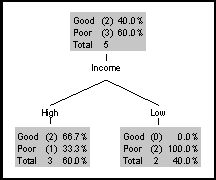
\includegraphics[width=0.3\textwidth]{img/sample_tree.jpg}
  \caption[labelInTOC]{Drzewo decyzyjne}
  \label{fig:sample_tree}
\end{center}
\end{figure}
\section{Drzewa decyzyjne}
% http://www.dbmsmag.com/9807m05.html
% When a businessperson needs to make a decision based on several factors, a
% decision tree can help identify which factors to consider and how each factor
% has historically been associated with different outcomes of the decision. For
% example, in our credit risk case study (See the sidebar Predicting Credit Risk),
% we have data for each applicant�s debt, income, and marital status. A decision
% tree creates a model as either a graphical tree or a set of text rules that can
% predict (classify) each applicant as a good or bad credit risk.

Kiedy biznesmen potrzebuje podj�� decyzje bazuj�c na kilku wsp�czynnikach,
drzewa decyzyjne mog� pomoc w wybraniu odpowiednich wsp�czynnik�w oraz 
opowiedzie� jak dany wsp�czynnik w przesz�o�ci wp�ywa� na decyzje.
Przyk�adowo, podczas obliczania ryzyka kredytowego, posiadamy dla ka�dego
potencjalnego kredytobiorcy dane o jego kredytach, przychodach oraz jego
statusie materialnym. Drzewa decyzyjne tworz� zar�wno drzewo w postaci
graficznej, jak zbi�r regu� tekstowych, dzi�ki kt�rym mo�emy okre�li�,
czy dana aplikacja jest obarczona du�ym lub ma�ym ryzykiem kredytowym.

% A decision tree is a model that is both predictive and descriptive. It is called
% a decision tree because the resulting model is presented in the form of a tree
% structure. (See Figure 1.) The visual presentation makes the decision tree model
% very easy to understand and assimilate. As a result, the decision tree has
% become a very popular data mining technique. Decision trees are most commonly
% used for classification (predicting what group a case belongs to), but can also
% be used for regression (predicting a specific value).

Drzewo decyzyjne jest modelem, kt�ry jest zar�wno predyktywnym!!!predictive and
descriptive!!!.
Nazywany jest drzewem decyzyjnym, poniewa� prezentowany jest w formie
drzewiastej struktury~\ref{fig:sample_tree}. Graficzna reprezentacja powoduje,
�e zrozumienie go czy por�wnanie go nie jest trudnym zadaniem. Drzewa decyzyjne
sta�y si� bardzo popularne w technikach ,,data maning''. Drzewa decyzyjne s�
najpowszechniej u�ywane do klasyfikacji (predykuj� do kt�rej grupy nale�y dany
przypadek), lecz mog� by� r�wnie� u�ywane przy regresji (predykuj� warto��).

% The decision tree method encompasses a number of specific algorithms, including
% Classification and Regression Trees (CART), Chi-squared Automatic Interaction
% Detection (CHAID), C4.5 and C5.0 (from work by J. Ross Quinlan of Rulequest
% Research Pty Ltd, in St. Ives, Australia, www.rulequest.com).

Metody drzew decyzyjnych obejmuj� wiele algorytm�w. Mi�dzy innymi drzewa
klasyfikuj�ce i regresyjne (ang. \emph{Classification and Regression Trees
(CART)}), \emph{Chi-squared Automatic
Interaction Detection (CHAID)}, \emph{C4.5} and \emph{C5.0}.

% Decision trees graphically display the relationships found in data. Most
% products also translate the tree-to-text rules such as If Income = High and
% Years on job > 5 Then Credit risk = Good. In fact, decision tree algorithms are
% very similar to rule induction algorithms which produce rule sets without a
% decision tree.

Drzewa decyzyjne w graficzny spos�b obrazuj� zale�no�ci wyst�puj�ce w danych.
Mo�na je r�wnie� przedstawia� w postaci regu� tekstowych np.
\\
\\
\emph{Je�li Doch�d = Wysoki i Lata Pracy $>$ 5 Wtedy Ryzyko kredytowe = Ma�e}.
\\
\\
Algorytmy drzew decyzyjnych s� bardzo podobne do algorytm�w indukcji regu�, kt�re
produkuj� zbiory regu� bez drzew decyzyjnych.

% The primary output of a decision tree algorithm is the tree itself. The 
% training process that creates the decision tree is usually called induction. 
% Induction requires a small number of passes (generally far fewer than 100) 
% through the training dataset. This makes the algorithm somewhat less efficient 
% than Na�ve-Bayes algorithms (See Na�ve-Bayes and Nearest Neighbor.), which 
% require only one pass, but significantly more efficient than neural nets, which 
% typically require a large number of passes, sometimes numbering in the 
% thousands. To be more precise, the number of passes required to build a 
% decision tree is no more than the number of levels in the tree. There is no 
% predetermined limit to the number of levels, although the complexity of the 
% tree as measured by the depth and breadth of the tree generally increases as 
% the number of independent variables increases.

G��wny rezultatem algorytmu drzew decyzyjnych jest w�a�nie drzewo. Proces
treningu tworzy drzewo, jest zwyczajowy nazywany indukcj�. Indukcja wymaga kilku
przej�� (generalnie znacznie mniej ni� 100) przez zbioru trenuj�cy (eg.
training dataset). Powoduje to, �e algorytmy te s� mniej wydajne ni� algorytmy 
\emph{Na�ve-Bayes}, kt�re wymagaj� tylko jednego przej�cia, ale znacznie wydajne
ni� sieci neuronowe, kt�re zazwyczaj wymaj� wielkiej ilo�ci przej��, czasami
liczonych w tysi�cach. Dok�adniej ilo�� ilo�� potrzebnych przej�� wymaganych do
zbudowania drzewa decyzyjnego jest nie wi�ksza ni� wysoko�� drzewa (ilo��
warstw). Nie istnieje okre�lona z g�ry maksymalna wysoko�� drzewa, jednak�e
z�o�ono�� drzewa mierzona jako jego wysoko�� i szeroko�� generalnie ro�nie je�li
ro�nie ilo�� niezale�nych zmiennych.


%\usepackage{graphics} is needed for \includegraphics
\begin{figure}[htp]
\begin{center}
  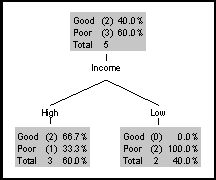
\includegraphics[width=0.3\textwidth]{img/sample_tree.jpg}
  \caption[labelInTOC]{Drzewo decyzyjne}
  \label{fig:sample_tree}
\end{center}
\end{figure}

\subsection{Om�wienie algorytm�w}
O
\subsubsection{ID3}
I
\subsubsection{C4.5}
C
\chapter{Indukcyjne bazy danych}
\section{Indukcyjne bazy danych}

% przetlumaczone z~pdf-a
Indukcyjne bazy danych �ci�le integruj� bazy danych z~koncepcj� \emph{data mining}~(\ref{lab:data_mining}).
G��wn� ich ide� stanowi to, �e zar�wno dane jak i~wzorce s� przetwarzane 
w ten sam spos�b, a~indukcyjny j�zyk zapyta� pozwala u�ytkownikowi 
na zadawanie zapyta� i~manipulacj� danymi wzorcami.

Od pocz�tku istnienia idei data miningu zdawano sobie spraw�,
�e proces ich przetwarzania powinien by� wspierany przez technologi� baz danych.
W ostatnich latach idea ta zosta�a sformalizowana jako koncepcja
\emph{indukcyjnych baz danych}.

%cytat z~artykulu
Integracja technologii baz danych z~nowoczesnymi metodami
indukcyjnego generowania wiedzy jest naturalnym kierunkiem rozwoju
system�w bazodanowych. Systemy nazywane indukcyjnymi bazami
danych potrafi� odpowiedzie� nie tylko na pytania, dla kt�rych
odpowied� znajduje si� w~bazie danych, ale r�wnie� na pytania,
kt�re wymagaj� zsyntetyzowania i~zastosowania wiedzy,
wygenerowanej przez indukcyjne wnioskowanie z~fakt�w z~bazy danych
i wcze�niejszej wiedzy~\cite{knowledge_disc}. Schemat typowej indukcyjnej
bazy danych przedstawiony jest na rysunku~\ref{fig:inddb}.

\begin{figure}[!ht]
     \centering
         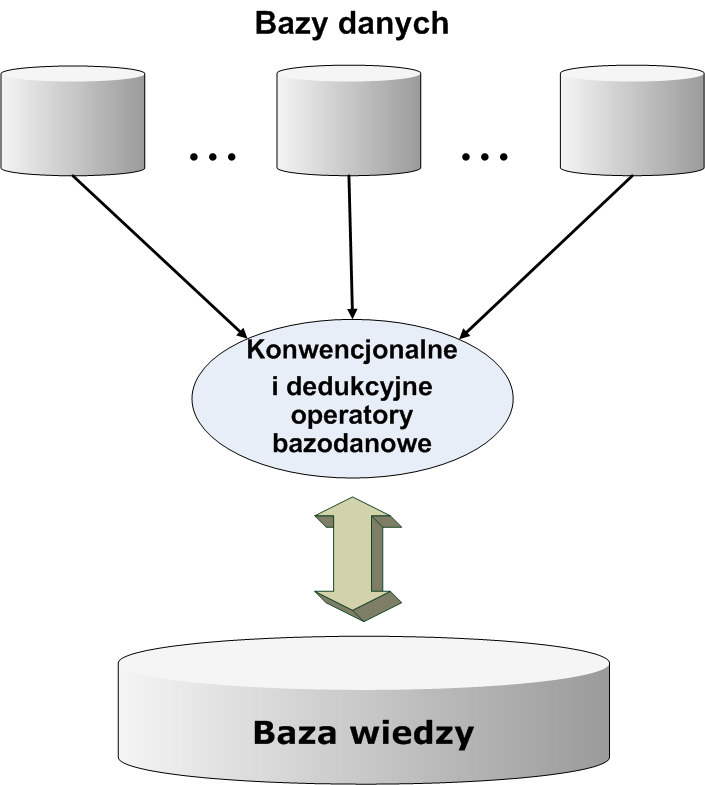
\includegraphics[width=0.90\textwidth]{img/knowledge_mining.png}
     \caption{Indukcyjna baza danych~\cite{ind_databases}}
     \label{fig:inddb}
\end{figure}

Jak zosta�o ju� wy�ej wspomniane, indukcyjne bazy danych przechowuj� nie dane
ale r�wnie� wzorce. Mo�na za�o�y�, �e zar�wno dane, jak i~wzorce stanowi� zbiory zbior�w.
To za�o�enie wynika z~analogii do tradycyjnych, relacyjnych baz danych. 
Relacyjna baza danych zawiera zbi�r relacji, kt�re to~stanowi� zbiory \emph{tupli}, 
a wi�c mo�na powiedzie�, ze stanowi zbi�r zbior�w.

W przypadku baz indukcyjnych rozr�nia si� natomiast zbi�r trenuj�cy od testuj�cego, 
zbi�r poprawnie zaklasyfikowanych przyk�ad�w od zaklasyfikowanych b��dnie itp.
 
To samo, co tyczy si� danych, odnosi si� r�wnie� do wzorc�w.
I rzeczywi�cie -- podczas procesu przetwarzania wiedzy mo�na pracowa� 
na r�nych zbiorach wzorc�w.  Zbiory te mog� odnosi� si� do odmiennych hipotez 
stworzonych na podstawie r�nych zbior�w danych,
czy r�nych ustawie� parametr�w algorytm�w je tworz�cych.

%jezyk (z pdf-a)
Jednym z~zasadniczych powod�w, kt�re przyczyni�y si� do sukcesu relacyjnych baz danych
jest opracowanie uniwersalnego j�zyka zapyta�, kt�ry podobnie jak sama algebra relacyjna
dostarcza du�ych mo�liwo�ci przy jego relatywnej prostocie.

Podobnymi cechami powinien wyr�nia� si� j�zyk zapyta� do indukcyjnych baz danych.

Rezultatem zapytania wykonanego w~takim j�zyku jest albo zbi�r wzorc�w, albo zbi�r danych.
Jest to~tak zwana \emph{w�asno�� zamkni�cia} (\emph{ ang. closure property}).
Stanowi ona analogi� do rezultat�w zapytania do relacyjnych baz danych, gdzie jest nim zawsze relacja.
Rozr�nianie mi�dzy zbiorami wzorc�w i~zbiorami danych powoduje, �e potrzebne s� dwa rodzaje zapyta�:
te kt�re generuj� zbiory wzorc�w i~zbiory danych. Zapytania do jednocze�nie obu typ�w zbior�w nazywane
s� czasami \emph{zapytaniami krzy�uj�cymi} (\emph{ang. cross-over operations}).

%dodawanie/usuwanie data setow, patternow? (patternow trudniej, nie wiem dokladnie jak, olac na razie)

%wnioskowanie
% z~pdf-a
Teoria indukcyjnych baz danych mo�e by� u�yteczna tylko w~przypadku,
gdy oferuje mo�liwo�� wnioskowania z~danych i~zgromadzonej wiedzy.
Na podstawie otrzymanej informacji trenuj�cej indukcyjna baza danych generuje now� lub 
ulepsza wcze�niej posiadan� wiedz�, w~pewien ustalony spos�b reprezentowan� 
i przeznaczon� do wykorzystania przy wykonywaniu okre�lonego zadania.
Mechanizm, zgodnie z~kt�rym dokonuje si� nabywanie lub doskonalenie wiedzy, 
jest najcz�ciej jednoznacznie wyznaczany przez metod� reprezentacji 
wiedzy oraz posta� informacji trenuj�cej \cite{ind_databases}.

\subsection{VINLEN}
\label{lab:vinlen}
Vinlen  \cite{vinlen} to system indukcyjnej bazy danych, rozwijany w
\emph{George Mason University}. Jest to~klasyczna
realizacja indukcyjnej bazy danych. Mechanizmy wnioskowania
indukcyjnego s� zintegrowane ze standardowymi relacyjnymi
operatorami bazodanowymi. Integracja ta opiera si� na nowych
rodzajach operator�w zwanych operatorami generowania wiedzy
\emph{KGO} (Knowledge Generation Operators). \emph{KGO} operuje na
\emph{segmentach wiedzy} sk�adaj�cych si� z~kombinacji jednej lub
wi�cej tabel z~relacyjnej bazy danych i~wiedzy przechowywanej
w~bazie wiedzy (por. rysunek~\ref{fig:inddb}). \emph{KGO} przyjmuje
na wyj�ciu jeden lub wi�cej segment wiedzy, na podstawie kt�rego
generuje inny segment wiedzy. Podstawowym operatorem u�ywanym w
systemie jest AQ21, program do indukcyjnego tworzenia regu� na
podstawie danych.

Indukcyjne bazy danych mog� by� wspierane przez wyspecjalizowanych
agent�w (\emph{Scauts}), kt�rych zadaniem jest synteza
i~zarz�dzanie wiedz�, kt�ra jest dostosowywana do wymaga�
okre�lonego u�ytkownika. System \emph{VINLEN} pozwala na tworzenie skrypt�w
operuj�cych na bazach danych, wiedzy i~algorytmach uczenia
maszynowego przy u�yciu j�zyka \emph{KGL-1} (\emph{Knowledge
Generation Language}).

Cech� charakterystyczn� tak rozwijanego systemu b�dzie mo�liwo��
sk�adowania wiedzy w~relacyjnej bazie danych wraz z~danymi,
zadawanie zapyta� oraz manipulowanie wiedz� z~wykorzystaniem
j�zyka \emph{KQL} lub przy u�yciu funkcjonalnego, graficznego
interfejsu u�ytkownika.



\section{Prace pokrewne}

\subsection{VINLEN}
to system indukcyjnej bazy danych, rozwijany w
\emph{George Mason University}~\cite{bib2}. Jest to klasyczna
realizacja indukcyjnej bazy danych. Mechanizmy wnioskowania
indukcyjnego s� zintegrowane ze standardowymi relacyjnymi
operatorami bazodanowymi. Integracja ta opiera si� na nowych
rodzajach operator�w zwanych operatorami generowania wiedzy
\emph{KGO} (Knowledge Generation Operators). \emph{KGO} operuje na
\emph{segmentach wiedzy} sk�adaj�cych si� z~kombinacji jednej lub
wi�cej tabel z relacyjnej bazy danych i~wiedzy przechowywanej
w~bazie wiedzy (por. rysunek~\ref{fig:inddb}). \emph{KGO} przyjmuje
na wyj�ciu jeden lub wi�cej segment wiedzy, na podstawie kt�rego
generuje inny segment wiedzy. Podstawowym operatorem u�ywanym w
systemie jest AQ21, program do indukcyjnego tworzenia regu� na
podstawie danych.

Indukcyjne bazy danych mog� by� wspierane przez wyspecjalizowanych
agent�w (\emph{Scauts}), kt�rych zadaniem jest synteza
i~zarz�dzanie wiedz�, kt�ra jest dostosowywana do wymaga�
okre�lonego u�ytkownika. System \emph{VINLEN} pozwala na tworzenie skrypt�w
operuj�cych na bazach danych, wiedzy i algorytmach uczenia
maszynowego przy u�yciu j�zyka \emph{KGL-1} (\emph{Knowledge
Generation Language}).

Cech� charakterystyczn� tak rozwijanego systemu b�dzie mo�liwo��
sk�adowania wiedzy w~relacyjnej bazie danych wraz z danymi,
zadawanie zapyta� oraz manipulowanie wiedz� z~wykorzystaniem
j�zyka \emph{KQL} lub przy u�yciu funkcjonalnego, graficznego
interfejsu u�ytkownika.

\subsection{Weka}
to narz�dzie do prowadzenia eksperyment�w
zwi�zanych z~uczeniem maszynowym stworzone w \emph{Uniwersity of
Waikato}~\cite{weka}. Narz�dzie to znajduje szerokie zastosowanie
w dydaktyce i badaniach naukowych. Mo�e r�wnie� udost�pnia� swoj�
funkcjonalno�� innym programom. Stanowi ono zbi�r narz�dzi do
zarz�dzania danymi w r�norodnych formatach, algorytm�w uczenia
maszynowego i~oceniaj�cych uzyskiwane rozwi�zania a~tak�e
�rodowisko do por�wnywania r�nych algorytm�w. �rodowisko zapewnia
przyjazny interfejs u�ytkownika, co czyni je �atwym
w~wykorzystaniu.

\emph{Weka} pozwala na wykorzystywanie r�norodnych �r�de� danych,
pocz�wszy od plik�w tekstowych w wielu formatach, poprzez
relacyjne bazy danych po dane umieszczone w Internecie. Dane te
przetwarzane s� przez tzw. \emph{filtry}, kt�re pozwalaj� na
wyodr�bnienie z nich potrzebnych informacji i przedstawienie ich w
czytelnej postaci.

Najwi�ksz� grup� algorytm�w zaimplementowanych w programie
\emph{Weka} s� algorytmy klasyfikuj�ce. Wykorzystuj� one wiele
form reprezentacji nauczonej wiedzy: od drzew i~regu� decyzyjnych,
przez maszyny wektorowe po sieci Bayesowskie.

Inn� grup� algorytm�w s� algorytmy grupuj�ce (klastruj�ce). Bazuj�
one na schematach \emph{k-Means}, \emph{EM}, \emph{Cobweb},
\emph{X-means}, \emph{FarthestFirst}. Utworzone za ich pomoc�
klastry mog� by� wizualizowane oraz por�wnywane do wzorcowych,
je�li takie s� do dyspozycji.

System \emph{Weka} implementuje r�wnie� popularny algorytm
\emph{Apriori}, wykorzystywany do znajdowania regu� asocjacyjnych.
Dzia�a on tylko na danych dyskretnych i pozwala na identyfikacj�
zale�no�ci statystycznych mi�dzy r�nymi grupami atrybut�w.

\emph{Weka} dostarcza przyjazny graficzny interfejs u�ytkownika,
kt�ry jest bardzo u�yteczny w praktyce.
Pozwala on nie tylko na sprawne wczytywanie danych do systemu,
ale tak�e na ich wizualizacj� w formie czytelnych diagram�w i~wykres�w.

Jedn� z ciekawszych funkcji systemu jest mo�liwo�� graficznego
definiowania przep�ywu danych i sposobu ich przetwarzania. �r�d�a
danych, filtry, klasyfikatory i algorytmy oceniaj�ce mog� by�
��czone graficznie za pomoc� linii. W~ten spos�b mo�na okre�la�
jaki ma by� przep�yw danych w systemie. Konfiguracja konkretnych
danych i metod ich przetwarzania mo�e by� zapisania i za�adowana
ponownie do powt�rnego wykorzystania.

\subsection{YALE}
(Yet Another Learing Environment), podobnie jak
opisywana powy�ej \emph{Weka}, jest systemem do prowadzenia
eksperyment�w zwi�zanych z uczeniem maszynowym.

Jego g��wn� zalet� jest bogaty zestaw operator�w, kt�re
umo�liwiaj� tworzenie ,,�a�cuch�w'' z�o�onych z r�nych problem�w
zwi�zanych z~uczeniem. Dane, na kt�rych operuj� operatory s� dla
nich ca�kowicie prze�roczyste i przechowywane mog� by� w
r�norodnych formatach -- za odpowiednie transformacje pomi�dzy
nimi odpowiada samo �rodowisko.

Dzi�ki operatorom i mo�liwo�ci ich �atwego ��czenia przy u�yciu
graficznego interfejsu u�ytkownika, a tak�e dzi�ki j�zykowi
skryptowemu bazuj�cemu na \emph{XML}, \emph{YALE} jest cz�sto
u�ywane do prowadzenia bada� i~eksperyment�w z r�norodnymi
algorytmami uczenia maszynowego.

\emph{YALE} dostarcza ponad 200 operator�w, jak cho�by algorytmy
klasyfikuj�ce, asocjacyjne, klastruj�ce, wyszukuj�ce regu�y czy
oparte na drzewach decyzyjnych. Dodatkowo mo�liwe jest
wykorzystanie wielu algorytm�w dostarczanych przez �rodowisko
\emph{Weka} w spos�b analogiczny do operator�w wbudowanych. Przed
przetworzeniem dane mog� by� poddane dyskretyzacji, filtrowaniu
czy normalizacji, a po zako�czeniu oblicze� odpowiedniej
walidacji.

\emph{YALE} pozwala na eksperymentowanie i~poszukiwanie najlepszego dla danego problemu
po��czenia r�nych metod uczenia maszynowego. Dzi�ki modularnej strukturze operator�w
mo�liwa jest wymiana pojedynczych ogniw ,,�a�cuch�w'' oblicze� w celu uzyskania
najlepszego efektu. Dodatkowo ,,�a�cuchy'' te mog� by� zagnie�d�ane, tworz�c skomplikowane
drzewa operator�w.



\chapter{Salomon}
\section{Powody powstania Salomona}

%Do czego ma byc to system?
%Istnieja inne...

%1. Struktura rozdzialu 2-giego powinna wygladac tak:
%- do czego ma byc system? (krotko, kilka zdan)
%- jaki ma byc? Czyli te akapity z wymaganiami, ale w innej kolejnosci:
%* ergonomia (prosty, przyjazny interfejs, API)
%* wlasny  sposob reprezentacji wiedzy (m.in. datasety wielowymiarowe)
%* wykorzystanie gotowych algorytmow (np. z Weki) i arch. komponentowa
%* rownoleglosc i rozproszenie
%* bezpieczenstwo
%* licencja
 
%Na koniec dochodzimy do wniosku, ze system powinien miec np. architekture komponenowa, napisany w Javie czy cos takiego.
 
%Kazdy z tych punkcikow oznaczonych '*' powinien miec mniej wiecej taka strukture:
%- jakiej cechy zadamy? (czyli np. "Jednym z postawowych zalozen stawianych systemowi jest prosty i przyjazny interfejs uzytkownika...")
%- dlaczego? ("Przyjazny interfejs ulatwia uzycie aplikacji zwlaszcza mniej doswiadczonym uzytkownikom...")
%- ewentualnie w zestawieniu z istniejacymi systami (Weka ma fajny, Vinlen niewygodny czy cos takiego)

%-gui
Jednym z podstawowych za�o�e� stawianych systemowi jest prosty i przyjazny interfejs u�ytkownika.

Cz�sto cech� decyduj�c� o rozpocz�ciu u�ywania danej aplikacji jest pierwszy kontakt z nia.
Dlatego wa�ne jest, aby graficzny interfejs u�ytkownika
u�atwia� u�ycie aplikacji mniej do�wiadczonym u�ytkownikom i aby nowy u�ytkownik naszego 
systemu nie zosta� zniech�cony ju� na samym pocz�tku.
Nale�y zatem zwr�ci� uwag�, by aplikacja by�a prosta w obs�udze zar�wno dla tw�rcy wtyczek
jak i osoby wykonuj�cej eksperymenty z wykorzystaniem gotowych wtyczek.
System powinien te� by� dostarczany z przyk�adowym zestawem wtyczek i danych, 
kt�re pozwol� na �atwe u�ycie i przetestowanie ka�dego z aspekt�w platformy.

%-api
Opr�cz przyjaznego graficznego interfejsu u�ytkownika platforma powinna
tak�e dostarcza� prostego i dobrze zdefiniowanego \emph{API}.
Pozwoli to na ukrycie przed tw�rcami wtyczek takich aspekt�w implementacyjnych
jak spos�b reprezentacji drzew decyzyjnych czy zapis parametr�w wej�ciowych i rezultat�w wykonania zada�.
Wynika to z tego, �e osoby, kt�re zajmuj� si� tworzeniem wtyczek 
nie powinny musie� bra� pod uwag� sposobu implementacji
platformy, czyli np. przechowywania i dost�pu do danych czy kwesti komunikacji
mi�dzy poszczeg�lnymi zadaniami.

Inn� u�yteczn� w�a�ciwo�ci�, kt�r� nale�y rozwa�y� jest 
umo�liwienie tworzenia wtyczek za pomoc� j�zyk�w skryptowych. Jest to 
szczeg�lnie po�yteczna w�a�ciwo�� np. w przypadku tworzenia nowego algorytmu.
W takiej sytuacji u�yteczna jest mo�liwo�� szybkiego wprowadzania zmian
i natychmiastowego przetestowania zachowania algorytmu bez koniczno�ci
prze�adowywania ca�ej wtyczki.

Wyspecyfikowanie dobrze zdefiniowanych interfejs�w pozwalaj�cych na manipulowanie wiedz�
pozwoli na znaczne uproszczenie procesu tworzenia wtyczek, a dodatkowo pozwoli na 
stworzenie wydajnego i dobrze przetestowanego API.

Z kolei ukrycie sposobu zapisu danych i wiedzy umo�liwi �atwiejsz� 
komunikacj� pomi�dzy r�nymi wtyczkami czy podsystemami. Odizolowanie 
algorytm�w (wtyczek) od zapisu/odczytu danych pozwoli r�wnie� zapewni� 
odpowiedni poziom bezpiecze�stwa. Przyk�adowo system powinien posiada� API 
pozwalaj�ce na tworzenie, manipulacje, odczyt i zapis drzew decyzyjnych, dzi�ki 
czemu r�ne aspekty pracy na drzewach decyzyjnych mo�na by by�o umie�ci� w 
osobnych wtyczkach, niekoniecznie dostarczanych przez tego samego dostawce. 
Jednak przede wszystkim praca nad jedn� cz�ci� (np. prezentacj� drzew) nie wymaga�oby 
wiedzy na temat innych wtyczek.

% - wiedza
System wspomagaj�cy procesy machine learningu, jakim ma by� nasza aplikacja,
powinien odznacza� si� sp�jnym i przejrzystym, a jednocze�nie wydajnym sposobem reprezentacji wiedzy.
Wi�kszo�� algorytm�w machine learning wymaga danych wej�ciowych.
Rozr�niamy dane trenuj�ce, kt�re s� wykorzystywane do uczenia algorytmu oraz 
dane testuj�ce. Zbi�r danych testuj�cych wykorzystywany jest do oceny wynik�w 
algorytmu. Oba zbiory zazwyczaj stanowi� losowy podzbi�r dost�pnych danych.

W znanych nam systemach u�ywan� s� jednowymiarowe zbiory trenuj�ce (jedna tabela, 
bez powi�za� z innymi). Taki model pasuje do wi�kszo�ci algorytm�w ucz�cych, jednak 
istnieje pewne ryzyko utraty danych, kt�re nios� z sob� relacje mi�dzy danymi. 
Dlatego chcieliby�my, aby nasz system tworzy� i operowa� na wielowymiarowych zbiorach 
trenuj�cych. Z punktu widzenie algorytmu struktura takiego zbioru nie powinna 
odbiega� od wej�ciowej bazy danych. Jedyna r�nica powinna polega� na ilo�ci 
dost�pnych danych. Takie te� jest pierwsze i najbardziej naturalne zrozumienie 
zbioru trenuj�cego, jako podzbioru danych o niezmienionej strukturze.

Nasz system powinien tworzy� podzbi�r danych przed utworzeniem atrybut�w.
Jest to podej�cie r�ne o tego, kt�re stosuje si� w innych aplikacjach.
Przyk�adowo w Wece zbi�r danych jest pozdbiorem zbioru atrybut�w. 
W naszym podej�ciu zbi�r danych nie b�dzie wymaga� kopiowania danych 
z zewn�trznego �r�d��, a jedynie definiowa� przepis na utworzenie takowego 
(np. w postaci zapytania, stanowi�cego zbi�r warunk�w).
Z kolej zbi�r atrybut�w stanowi� b�dzie opis transformacji oryginalnych danych
na dane wej�ciowe do algorytm�w ucz�cych. Wyr�nienie wartwy atrybut�w jest konieczne,
gdy� wi�kszo�� algorytm�w wymaga na wej�ciu przetworzonia danych.
Przetworzenie polega g��wnie na okre�leniu typu danego atrybutu, czyli np. czy jest to atrybut wej�ciowy
czy wyj�ciowy oraz jakiego jest rodzaju (napisowy, liczbowy, wyliczeniowy).

Rozwi�zanie przyj�te w naszym systemie zapewnia szereg korzy�ci. Atrybuty budowane na zbiorach danych umo�liwi�
zachowanie oryginalnej, cz�sto wielowymiarowej struktury oryginalnych danych i zwi�zk�w mi�dzy nimi.
Zastosowanie warstwy po�redniej mi�dzy atrybutami a danymi, w postaci zbior�w danych, ma te� inne zalety.
Poniewa� zbiory danych stanowi� jedynie opis, w jakis spos�b oryginalne dane mog� zosta� wydobyte
i jak maj� by� interpretowane, pozwala to na przechowywanie tych danych w zewn�trznych �r�d�ach.
Dzi�ki temu nie trzeba ich kopiowa� do bazy, na kt�rej maj� by� wykonywane algorytmy,
co wi��e si� z nie tylko z ich bezpiecze�stwem, ale tak�e pozwala algorytmom na prac� z zawsze aktualnymi
danymi bez konieczno�ci dodatkowej synchronizacji mi�dzy �r�d�ami danych, a aplikacj�, kt�ra z nich korzysta.
Nie bez znaczenia jest te� fakt, �e przechowuj�c dane w zewn�trznych �r�d�ach danych
i unikaj�c konieczno�ci ich kopiowania mo�na oszcz�dzi� sporo przestrzeni dyskowej,
co mo�e mie� du�e znaczenie przy pracy z ogromnymi zestawami danych.

% - architektura komponentowa
Jednym z podstawowych wymaga� stawianym naszemu systemowi, jest architektura komponentowa.
W celu poprawnego dzia�ania w wielkim rozproszonym 
�rodowisku, platforma uruchomieniowa powinna by� dobrze odseparowana od samych 
algorytm�w, co umo�liwi wsp�prac� w jednym �rodowisku r�nych wersji 
systemu, a nawet r�nych jego implementacji. Budowa systemu powinna w jak 
najwi�kszym stopniu wspiera� mo�liwo�� powstania r�nych niezale�nych 
implementacji algorytm�w uczenia maszynowego, dostarczanych przez r�nych 
dostawc�w. Dzi�ki odseparowaniu wtyczek od plaftormy i przeniesieniu na ni� 
odpowiedzialno�ci za zapewnienie komunikacji mi�dzy poszczeg�lnymi wtyczkami
mo�liwe b�dzie np. zastosowanie oblicze� r�wnoleg�ych i rozproszonych, 
bez dodatkowych wymaga� stawianych wtyczkom.

% gotowe algorytmy
Architektura komponentowa i niezale�no�� pomi�dzy poszczeg�lnymi wtyczkami 
umo�liwi wykorzystanie gotowych algorytm�w. W VINLENIE zosta�y cz�ciowo 
wykorzystane implementacje algorytm�w przygotowanych do wcze�niejszych 
projekt�w jak np. program Emerald (przypisek). Znajdziemy tam takie algorytmy jak 
Abacuse, AQ czy Cluster. Cz�� z tych implementacji jest bardzo nowatorska i dysponuje 
wielkimi mo�liwo�ciami. W Wece mo�emy znale�� jeszcze wi�ksz� gam� dost�pnych 
algorytm�w. Dlatego te� nasz system powinien charakteryzowa� si� odpowiednia 
architektur�, kt�ra w �atwy spos�b pozwala na powt�rne u�ycie ju� 
zaimplementowanych algorytm�w.
W przypadku u�ycia algorytm�w pochodz�cych z r�nych, nie zawsze pewnych �r�de�
pojawia si� problem bezpiecze�stwa oraz zaufania do r�nych 
implementacji. Naturalnym rozwi�zaniem tego problemu wydaj� si� zastosowanie 
bezpiecznych j�zyk�w programowania, takich jak Java wraz z jej systemem bezpiecze�stwa
i ograniczenia uprawnie�.

% - agenty (TODO:)
System powinien reagowa� na zmiany w �rodowisku, w kt�rym zosta� zainstalowany. 
Przyk�adowo, kiedy pojawiaj� si� nowe dane w zewn�trznej bazie danych, nale�y 
przetestowa� aktualnie zgromadzon� wiedz� na nowych danych lub dokona� nowych 
oblicze�. Jednym z innych wymaga� jest praca w rozproszonym �rodowisku i w tym 
przypadku ka�dy z agent�w mo�e niezale�nie wygenerowa� now� wiedze, po czym 
nowa wiedza powinna zosta� rozdystrybuowana do pozosta�ych agent�w. Takie 
podej�cie pozwala na bezobs�ugow� prace systemu. System sam powinien 
podejmowa� akacje w wyniku pewnych zdarze� w jego �rodowisku. Vinlen posiada 
wsparcie dla agent�w (zwanych tam skautami). Agenci w tym �rodowisku to 
integralna cz�� tego produktu. Weka nie posiada wsparcia dla takich 
mechanizm�w. Stanowi ona raczej narz�dzie do przeprowadzania akademickich 
eksperyment�w na algorytmach ni� narz�dzie do zastosowa� biznesowych, 
zainstalowane w �rodowisku produkcyjnym. Wa�ne, aby system posiada� cechy, 
kt�re umo�liwi� jego zastosowanie zar�wno rozwi�zaniach biznesowych jak i 
akademickich.

% - rownoleglosc i rozproszenie
System, kt�ry mo�e wykonywa� skomplikowane i d�ugotrwa�e obliczenia powinien
mie� mo�liwo�� ich rozpraszania.
W dobie rozpowszechniania si� technologi gridowych i klastrowych aplikacje powinny
m�c korzysta� z mo�liwo�ci, jakie te technologie udost�pniaj�.
Dzia�anie w �rodowisku heterogenicznym pozwala nie tylko na lepsze 
wykorzystanie zasob�w sprz�towych, ale r�wnie� na dost�p do wielu �r�de� danych 
przy zapewnieniu bezpiecze�stwach tych danych. Rozproszone instancje powinny 
wymienia� jak najmniejsz� ilo�� informacji, by nie obci��a� namiernie zasob�w komunikacyjnych.

Nasz system powinien tak�e umo�liwia� zr�wnoleglanie niekt�rych oblicze�.
Taka mo�liwo�� powinna by� dost�pna ramach pojedynczej instancji systemu,
co powinno by� uwzgl�dnione w jego architekturze.
W naszym przypadku w�a�ciwym i najprostszym modelem jest napisanie 
aplikacji pracuj�cych w oparciu o w�tki i przeniesienie ci�aru zrownolegniania 
na inne mechanizmy, takie jak klasteryzcja itp. Obecnie na rynku znajduj� si� systemy
pozowalaj�ce na zr�wnoleglenie aplikacji wielow�tkowej w spos�b prze�roczysty 
dla u�ytkownika jak i dla aplikacji. �wietnym przyk�adem takiej aplikacji jest 
np. MOSIX (http://www.mosix.org/), kt�ry z klastr�w linuxowych x86 tworzy 
system wieloprocesorowy.

W celu zapewnianiu bezpiecze�stwa danych, aplikacja nie powinna wysy�a� samych danych,
ale wy��cznie wiedz�. Nale�y r�wnie� za�o�y� ograniczone zaufanie do instancji 
pracuj�cych w nieznanym �rodowisku, dlatego ka�de �r�d�o danych powinno by� zabezpieczone.
W zastosowaniach komercyjnych system mo�e mie� dost�p do kluczowych danych 
przedsi�biorstwa czy instytucji. Model bezpiecze�stwa komunikacji mi�dzy 
r�nymi instancjami, chcieliby�my oprze� na obecnie dost�pnych metodach ochrony 
jak np. VPN (Virtual Private Network). Zak�adamy, �e nasz system b�dzie zainstalowany w 
bezpiecznym �rodowisku, dlatego ochron� warstwy komunikacji powinien 
zaj�� si� administrator.

% TODO: to gdzie? (do wykorzystania algorytmow?)
%Wa�nym aspektem jest dost�p do algorytm�w Weki, 
%ale tak�e do ewentualnego u�ycia algorytm�w z VINLENA, co jedna wymaga 
%zastosowania odpowiedniej licencji (link do odpowiedniego punktu. VINLEN zosta� 
%napisany w j�zyku C++, zatem system powinnen wspiera� r�wnie� inne j�zyki 
%programowania a szczeg�lnie wspomniany C++.

% TODO - to gdzie?
%Kolejnym aspektem architektury jest spos�b aktualizacji 
%algorytm�w. Je�li w przypadku samej platformy aktualizacja nie b�dzie 
%dokonywana cz�sto to jednak w przypadku algorytm�w mo�e to nast�powa� bardzo 
%cz�sto. Przyk�adowym zastosowaniem wymagaj�cym cz�stych aktualizacji jest 
%wynajmowanie mocy obliczeniowej innym instytucjom. Mo�na wyobrazi� sobie 
%sytuacje, w kt�rej nasz system zainstalowany jest na wydajnej maszynie, np. klastrze.
%Wykonuje on obliczenia na zlecenie, co w oczywisty spos�b 
%wymaga�oby pobrania nie tylko parametr�w, czy danych, ale r�wnie� samych 
%algorytm�w. Oba referencyjne systemy nie spe�niaj� wymaganych przez nas 
%kryteri�w.

% TODO: to gdzie?
%W odr�nieniu od innych system�w, szczeg�lny nacisk chcemy po�o�y� na 
%platform�, a nie na same algorytmy. Jak ju� wcze�niej zosta�o powiedziane, 
%wa�ne jest, aby da�o si� wykorzysta� gotowe implementacje algorytm�w machine 
%learning. W zwi�zku z tym bardzo wa�nymi aspektami s�: proste API (z ang. 
%Application Program Interface) oraz licencja (link do dalszej czesci?).

% -- Licencja
Istotn� cech� wp�ywaj�c� na popularno�� aplikacji jest spos�b ich licencjonowania,
dlatego nasz system powininen by� dost�pny na licencji, kt�ra umo�liwia� b�dzie jego
powszechne u�ywanie.
VINLEN to system komercyjny, dostarczany bez kodu �r�d�owego, 
dlatego jego wykorzystanie jest utrudnione zar�wno jako platformy dla w�asnych 
algorytm�w jak i jego algorytm�w. Z racji braku kodu �r�d�owego nie s� mo�liwe 
ewentualne modyfikacje i dostosowania do naszych potrzeb.
Weka dostarczana jest na licencji GPL, kt�ra jest licencj� open source, jednak r�wnie� stwarza pewne problemy. 
W przypadku tej licencji niemo�liwe jest u�ycie aplikacji w innym systemie o 
zamkni�tym kodzie �r�d�owym.
Licencja, na kt�rej b�dzie dost�pny nasz system powinna umo�liwia� wykorzystanie 
go w zamkni�tych, komercyjnych projektach, a zarazem po��dan� cech� jest to, 
aby by�a zgodna z GPL. Zgodno�� licencji jest wymagana do ewentualnego u�ycia 
algorytm�w Weki w naszym systemie. Po wst�pnej analizie dost�pnych licencji, 
jedn� z tych, kt�ra spe�nia nasze, wymagania jest licencja 
LGPL (wstawi� przypis i odno�niki).

% to moze pod koniec, we wnioskach do tego rozdzialu (jesli wogole to dawac)
% TODO - to gdzie?
%Po przeanalizowaniu obecnych narz�dzi do uczenia maszynowego stwierdzili�my, �e 
%dost�pne systemu tego typu posiadaj� pewne ograniczenia, kt�re chcieliby�my 
%wyeliminowa�. Po zapoznaniu z wieloma narz�dzami doszli�my do wniosku, �e 
%najbli�ej naszych wymaga� s� dwie aplikacje: VINLEN oraz Weka. Dlatego 
%omawiaj�c nasze wymagania, b�dziemy nawi�zywa� do tych dw�ch aplikacji. R�wnie� 
%dlatego, �e chcieliby�my, tworz�c nasz� aplikacje, wzorowa� si� na tych dw�ch 
%programach.  

%II. Salomon
%1. Napisa� postulaty - dlaczego piszemy Salomona:
%Funkcje:
%rozproszenie
%- wykorzystanie gotowych algorytm�w
%bezpiecze�stwo
%- komponentowa architektura
%- podej�cie do data set i attribute set
%- jedna reprezentacja wiedzy dzielona pomi�dzy ro�ne algorytmy
%- przeno�no��
%- dost�p nie tylko do wiedzy, ale tak�e do danych (indukcyjna baza danych)
%Api i licencja:
%- proste API
%- licencja
%

% \section{Powody powstania Salomona}
% Po przeanalizowaniu obecnie dost�pnych narz�dzi do uczenia maszynowego
% stwierdzili�my, �e oprzemy nas system na na dw�ch aplikacjach \emph{Weka}
% oraz \emph{Vinlen}. 
% 
% \subsection{Indukcyjne bazy danych}
% Przyk�adem indukcyjnej bazy danych jest system \emph{Vinlen}. Powsta� on jako 
% realizacja tej koncepcji. System ten s�u�y� nam jako wzorcowa implementacja. Z
% zwi�zku z pewnymi niedoskona�o�ciami tego rozwi�zania zdecydowali�my si� na
% stworzenie w�asnej implementacji. 
% 
% W dobie Internetu, coraz wi�cej aplikacji pracuje w �rodowisku rozproszonym.
% Znana nam wersja systemu Vinlen nie posiada�a mo�liwo�ci pracy w �rodowisku
% rozproszonym, co jednak uznali�my za powa�ny brak. Dwa g��wne powody
% przemawiaj�ce za rozproszeniem to lepsze wykorzystanie zasob�w (klasteryzacja)
% oraz dost�p do rozproszonych danych oraz wiedzy.
% 
% Vinlen jest rozwijany na uniwersytecie TUTAJ WSTAWI� NAZW� jako zamkni�ty
% produkt. My jednak postanowili�my udost�pni� nasz system na otwartej licencji
% \emph{LGPL}, kt�ra pozwala u�ywanie go jako biblioteki w komercyjnych
% produktach. Jednak w takim przypadku nie mo�na wykorzysta� integracji z Weka z
% racji na jej licencj� (GNU). Weka dostarcza implementacji wielu popularnych
% algorytm�w uczenia maszynowego, dlatego te� stwierdzili�my, �e zamiast
% dostarczenia w�asnej implementacji dostarczymy integracji z Wek�, przez co
% zyskamy dost�p do jej bogatej biblioteki gotowych algorytm�w. Vinlen korzysta z
% w�asnych implementancji algorytm�w, z kt�rych cz�� powsta�a na uniwersytecie !!!!!.

%TODO
%1. Rozproszenie
%2. Wykorzystanie gotowych algorytmow (vinlen wszystko sam pisze)
%3. Komponentowa architektura
%4. Proste API
%5. Otwarta licencja
%6. Podejscie do datasetow i atrybutow
%7. Jedna reprezentacja wiedzy (w wece drzewa nie maja wpolnej reprezentacji przez co niezaleznie rozwijane algorytmy moga ze soba wspolpracowac

%2. Uzasadnienie potrzeby stworzenia platformy
%	
%- dwa aspekty tematyki uczenia maszynowego:
%	* indukcyjne bazy danych (i Vinlen)
%	* eksperymenty i doswiadczenia (Weka itd.)
%- z tego ma wynikac koncepcja Salomona:
%	* jako platformy laczacej te aspekty
%	* odpowiedz na ograniczenia np. Vinlena
%- przedstawic postulaty, ktore spelaniac ma platfroma
%	* zalozenia koncepcyjne (np. koncepcja zadan)
%	* zalozenia implementacyjne (przenosnosc, rownoleglosc itp).

\chapter{Opis systemu}
\section{Wprowadzenie}

Salomon to system do wydobywania wiedzy z danych zgodnie z metodologi� \emph{Knowlege Mining}.
Odkrywanie wiedzy to proces iteracyjny, podzielony na etapy. W ka�dym tym etapie wiedza jest poddawana
obr�bce. Etapy te mog� tworzy� cykle. Na ka�dym takim etapie proces odkrywania mo�e by� ukierunkowany zgodnie
z wymaganiami u�ytkownika. Ka�dy etap tworzy odr�bn� ca�o��. 

W Salomonie reprezentacj� etapu jest \emph{zadanie} (Task). Ka�de zadanie mo�e posiada� kilka nast�pnik�w i kilka
poprzednik�w. Ujmuj�c rzecz pro�ciej, zadania mog� by� zorganizowane w postaci grafu. 

Zadanie zdefiniowane jest jako tr�jka:
\begin{itemize}
	\item algorytm(dostarczany w postaci wtyczki, czyli \emph{pluginu}))
	\item dane steruj�ce algorytmem
	\item dane wej�ciowe, z kt�rych algorytm b�dzie wydobywa� wiedz�
\end{itemize}

Zadanie nie musi si� ogranicza� do danych, kt�re otrzyma�o z poprzedniego zadania. Ka�de zadanie ma
dost�p do ca�ej aktualnie zgromadzonej wiedzy i do wszystkich danych.

Na wej�ciu lub wyj�ciu ka�dego zadania mog� pojawi� si� dane (w przypadku algorytm�w, kt�re
dokonuj� selekcji/segregacji danych), wiedza lub obie te rzeczy naraz.

\begin{itemize}
	\item dane \begin{math}\Rightarrow \end{math} dane - najcz�ciej taki przypadek zdarza si� kiedy chcemy stworzy�
	zbiory treningowe lub zbiory testuj�ce
	\item dane \begin{math}\Rightarrow \end{math} wiedza - typowy przyk�ad wyszukiwania wiedzy: dostajemy dane, uzyskujemy wiedz�
	\item wiedza+dane \begin{math}\Rightarrow \end{math} dane - przypadek taki zachodzi kiedy chcemy wykorzysta� zgromadzon� wiedz� na dostarczonych danych
	\item wiedza \begin{math}\Rightarrow \end{math} wiedza
\end{itemize}

Celem tego projektu jest stworzenie przyjaznego �rodowiska do tworzenia, kontrolowania i efektywnego wykonywania zada� oraz przechowywania zgromadzonej wiedzy.

Salomon sk�ada si� z dw�ch zasadniczych cz�ci - pierwsz� z nich
stanowi platforma. Tworz� j�:
\begin{itemize}
	\item silnik, kt�rego zadaniem jest zarz�dzanie i~uruchamianie
zada�
	\item magazyn s�u��cy do przechowywania wiedzy
\end{itemize}

Druga cz�� to zbi�r wtyczek, dostarczaj�cych logik� potrzebn� do skonfigurowania, wykonania i~wy�wietlenia rezultat�w
zadania. System jest otwarty - oznacza to, �e jego funkcjonalno�� mo�e by� w �atwy spos�b rozszerzana poprzez dostarczenie nowych wtyczek.

\begin{figure}[htb]
	\centering
		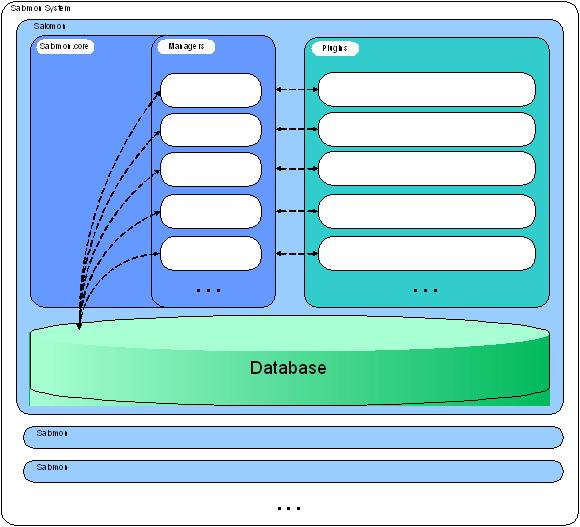
\includegraphics[width=0.90\textwidth]{img/uml/arch.jpg}
	\caption{Architektura systemu}
\end{figure}


\pagebreak
Podstawowe za�o�enia projektowe:
\begin{itemize}
    \item ca�a funkcjonalno�� w pluginach. J�dro systemu ma by� jak najmniejsze.
    Jego zadaniem jest stworzenie �rodowiska do realizacji logiki dostarczanej we wtyczkach
    \item otwarta~architektura. Wprowadzenie warstwy po�redniej pomi�dzy baz� danych~a wtyczkami.
    Jej zadaniem jest ukrycie sposobu organizacji danych przez
    wtyczkami. Otwarto��~architektury polega na mo�liwo�ci rozszerzenia tej warstwy
    \item niezale�no�� od platformy. System ma by� niezale�ny od platformy, mo�liwie �atwo przenaszalny.
    Poszczeg�lne cz�ci systemu mog� by� uruchamiane na r�nych
    platformach.
    \item mo�liwo�� wykorzystywania rezultat�w poprzednich zada� przez kolejne
    \item �atwa~adaptacja funkcjonalno�ci zawartej w \emph{Vinlenie}.
    Projekt powsta� jako platforma uruchomieniowa dla logiki zaimplementowanej w programie \emph{Vinlen},
    tworzonego pod kierownictwem prof. Ryszarda Michalskiego.    
\end{itemize}


Salomon ma na celu wyeliminowanie ogranicze� oryginalnego
\emph{Vinlena} poprzez wprowadzenie:

\begin{itemize}
    \item kolejkowania zada�
    \item rozproszenia
    \item r�wnoleg�o�ci
    \item rozszerzalno�ci (mechanizm wtyczek)
    \item przeno�no�ci (\emph{Java},\emph{Firebird})
\end{itemize}
\section{Koncepcja systemu}

Przedstawiona poni�ej koncepcja zak�ada stworzenie systemu o~nazwie \emph{Salomon}, kt�ry stanowi� b�dzie odpowiedz na opisane wcze�niej wymagania. 

Podstawowym za�o�eniem przy�wiecaj�cym opracowywaniu tego �rodowiska jest koncepcja zadaniowo�ci. \\
Odkrywanie wiedzy to~proces iteracyjny, podzielony na etapy. Etapy te mog� tworzy� cykle.
W ka�dym tym etapie wiedza jest poddawana obr�bce. 
Na ka�dym takim etapie proces odkrywania mo�e by� ukierunkowany zgodnie
z wymaganiami u�ytkownika. Ka�dy etap tworzy odr�bn� ca�o��. 
Cz�� etap�w jest roz��czna, zatem mog� by� wykonywane wsp�bie�nie. 
Architektura Salomona pozwala na rozproszone, a~co za tym idzie 
-- zr�wnoleglenie wykonywania takich roz��cznych etap�w oraz na synchronizacj� ich wynik�w.

Jednym z~istotnych atut�w systemu jest mo�liwo�� elastycznego definiowania
przebiegu pracy systemu w~kategoriach tzw.\ \emph{zada\'n}.
Ekstrakcja wiedzy to~proces, kt�ry mo�e
by� podzielony na etapy -- w~ka�dym etapie wiedza jest poddawana
pewnej obr�bce (np. dyskretyzowane s� atrybuty, tworzone s�
regu�y, wiedza jest testowana). Poniewa� ka�dy etap tworzy odr�bn�
ca�o��, a~cz�� etap�w jest od siebie niezale�na, zatem mog� by�
one wykonywane wsp�bie�nie.

\label{lab:tasks}
Zadanie to~podstawowa jednostka reprezentuj�ca obliczenia.
Zdefiniowane jest ono jako: 
$$
z=(a, p, we, wy)
$$
gdzie:
\begin{itemize}
    \item $a$ jest algorytmem, dostarczanym do systemu w~postaci komponentu --
    wtyczki,
    \item $p$ reprezentuje parametry algorytmu,
    \item $we$ i~$wy$ oznaczaj� odpowiednio informacje wej�ciowe i
    wyj�ciowe algorytmu.
\end{itemize}
Wej�cie i~wyj�cie mo�e mie� posta� danych (w~przypadku algorytm�w,
kt�re dokonuj� np. selekcji danych), wiedzy (np. wygenerowane
regu�y) lub danych i~wiedzy naraz (np.\ regu�y i~wyj�tki dla
nich).

Wyj�cie jednego zadania mo�e by� wej�ciem pewnej liczby nast�pnych
zada�. Aby zadanie mog�o zosta� wykonane, wszystkie zadania od
kt�rych zale�y musz� by� wykonane wcze�niej. Powi�zane zadania
mog� by� przedstawione w~postaci grafu skierowanego. Taki graf z
zaznaczonym zadaniem pocz�tkowym tworzy \emph{program}. Dodatkowo,
ka�da kraw�d� mo�e mie� przypisany warunek, kt�ry jest wymagany,
aby sterowanie zosta�o przekazane wzd�u� tej kraw�dzi. Tak
zdefiniowany program mo�e by� �atwo prezentowany u�ytkownikowi w~postaci
graficznej. 

\label{lab:agents}
W systemie mo�na definiowa� agent�w, kt�rzy reaguj� na zmiany w~danych i/lub
wiedzy. Obecnie jest jedynym rodzajem zdarzenia, kt�ry mo�e wywo�a� akcje
jest pojawienie si� nowych danych w~systemie. Jednak w~przysz�o�ci istnieje
mo�liwo�� dodania kolejnych rodzaj�w zdarze� takich jak np. wygenerowanie
wiedzy przez innego agenta. W~reakcji na wyst�pienie zdarzenia system
wykonuje zdefiniowany program, za pomoc� kt�rego mo�na przyk�adowo sprawdzi� poprawno�� aktualnej zgromadzonej wiedzy na nowych danych, czy wygenerowa� now�.
% (np.\ na dodanie nowego rekordu do danych treningowych, czy
%wygenerowanie wiedzy przez innego agenta).
%W~systemie b�dzie mo�na tak�e
%definiowa� agent�w, kt�rzy reagowa� b�d� na zmiany w~danych i/lub wiedzy
%(np.\ na dodanie nowego rekordu do danych treningowych, czy
%wygenerowanie wiedzy przez innego agenta).


%W~systemie b�dzie mo�na tak�e
%definiowa� agent�w, kt�rzy reagowa� b�d� na zmiany w~danych i/lub wiedzy
%(np.\ na dodanie nowego rekordu do danych treningowych, czy
%wygenerowanie wiedzy przez innego agenta).

Bardzo wa�nym mechanizmem Salomona jest mo�liwo�� tworzenia powi�za� 
mi�dzy poszczeg�lnymi zadaniami. 
Wynik jednego zadania mo�e pos�u�y� jako wej�cie nast�pnego. 
Salomon w~tym celu dostarcza �rodowisko. Wtyczka w~trakcie wykonywania zadania 
opr�cz dost�pu  do menad�er�w posiada r�wnie� dost�p do �rodowiska, 
z kt�rego mo�e pobra� warto�ci zmiennych �rodowiskowych. 
Dane �rodowisko tworzone jest na pocz�tku wykonania listy zada� 
i przekazywane jest kolejno do nast�pnego zadania. 
Wtyczka w~trakcie pracy mo�e modyfikowa� �rodowisko poprzez dodawanie, 
usuwanie oraz edycj� poszczeg�lnych zmiennych. W~ten spos�b poszczeg�lne 
zadania mog� mi�dzy sob� przekazywa� informacje. Zmienne �rodowiskowe, 
podobnie jak ustawienia i~rezultaty zada�, s� persystentne, a~co za tym 
idzie potrzebny jest mechanizm serializacji i~deserializacji.

Mechanizm tworzenia zmiennych �rodowiskowych opiera si� na tym samym modelu
co tworzenie ustawie� i~rezultat�w dla zada�. Mo�liwo�� tworzenia zmiennych
�rodowiskowych przez wtyczki mo�e rodzi� wiele problem�w z~zapewnieniem 
kompatybilno�ci mi�dzy r�nymi wersjami wtyczek, komunikuj�cych si� ze sob�, 
dlatego te� aby unikn�� takich problem�w, ka�da wtyczka zmuszona b�dzie 
dostarczy� opis zmiennych, kt�re mo�e tworzy�.

% TODO: przeniesc do implementacji -- dodac cos o~serializacji
%Mechanizm serializacji opiera si� na agregacji typ�w prostych 
%i innych typ�w z�o�onych. Za~pomoc� takich element�w, 
%programista mo�e stworzy� hierarchiczne struktury danych.
%Wprowadzenie takiego mechanizmu podyktowane jest potrzeb� ukrycia
%przed programist� sposobu zapisu danych w~bazie lub w~pliku. 
%Dostarczenie sp�jnego modelu serializacji danych pozwala na 
%niewidoczny dla wtyczek spos�b podmiany implementacji na bardziej 
%efektywn� itp. Mechanizm ten mo�e okaza� si� r�wnie� po�yteczny 
%po dodaniu do Salomona mo�liwo�ci definiowania zada� w~pliku (np. XML).
%Serializacja danych mo�e odbywa� si� do wielu format�w 
%np. XML, CSV, tabel w~bazie danych itp.

Na wej�ciu lub wyj�ciu ka�dego zadania mog� pojawi� si� dane (w przypadku algorytm�w, kt�re
dokonuj� selekcji/segregacji danych), wiedza lub obie te rzeczy naraz (rys. \ref{fig:WorkflowGraph} i~rys. \ref{fig:WorkflowSequental}).

\begin{itemize}
	\item \begin{math} dane \Rightarrow  dane \end{math} - najcz�ciej taki przypadek zdarza si� kiedy chcemy stworzy�
	zbiory treningowe lub zbiory testuj�ce
	\item \begin{math} dane \Rightarrow wiedza \end{math} - typowy przyk�ad wyszukiwania wiedzy: dostajemy dane, uzyskujemy wiedz�
	\item \begin{math} wiedza + dane \Rightarrow  dane \end{math} - przypadek taki zachodzi kiedy chcemy wykorzysta� zgromadzon� wiedz� na dostarczonych danych
	\item wiedza \begin{math}\Rightarrow \end{math} wiedza
\end{itemize}

\begin{figure}[H]
	\centering
		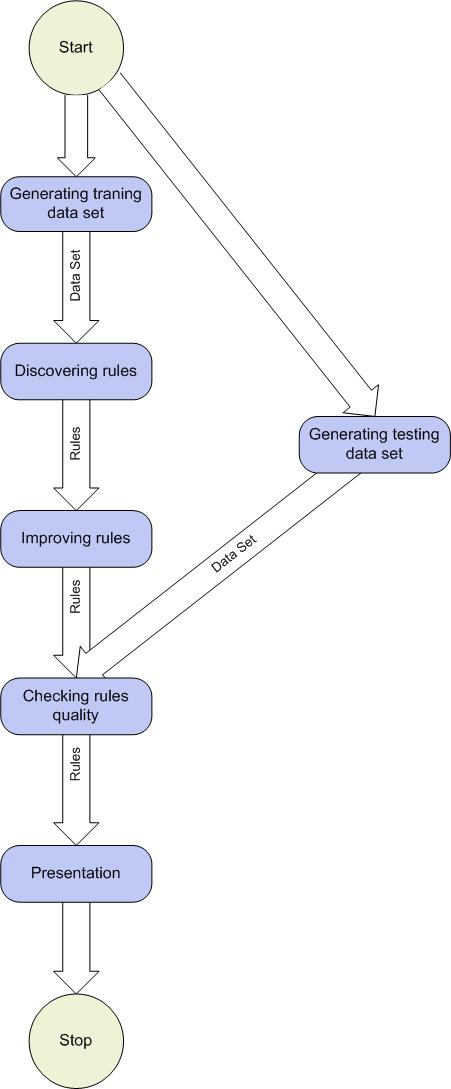
\includegraphics[height=0.90\textheight]{img/salomon/concept/WorkflowGraph.jpg}
	\caption{Przep�yw danych}		
	\label{fig:WorkflowGraph}
\end{figure}


\begin{figure}[H]
	\centering
		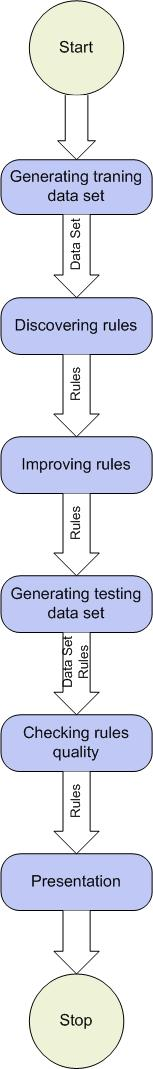
\includegraphics[height=0.90\textheight]{img/salomon/concept/WorkflowSequental.jpg}
	\caption{Sekwencyjny przep�yw danych}
	\label{fig:WorkflowSequental}
\end{figure}


\section{Funkcjonalno��}

Ca�a funkcjonalno�� \emph{Salomona} podporz�dkowana jest tworzeniu zada�. Operacje podstawowe, takie jak np. tworzenie projekt�w czy definiowanie wtyczek s�u�� jedynie stworzeniu �rodowiska, w~kt�rym mog� by� wykonywane zadania. Z~kolei operacje administracyjne pozwalaj� na~zaawansowane zarz�dzanie platform� i~mog� by� u�yteczne dla u�ytkownik�w bardzo dobrze znaj�cych wewn�trzn� struktur� systemu.

\subsection{Operacje podstawowe}

\subsubsection{Operacje na~obiekcie Solution}
\label{lab:solution}

Terminem \textbf{Solution} okre�lamy struktur� grupuj�c� projekty.
W obr�bie jednego obiektu \emph{Solution} zgrupowane s� projekty, 
kt�re operuj� na~tym samym zewn�trznym �r�dle danych.
W obecnej wersji s� to~zewn�trzne bazy danych. Obiekt ten przechowuje 
informacje niezb�dne do~uzyskania dost�pu do~danych,
a wi�c parametry po��czenia i~lokalizacj� bazy danych.

Mo�na na~nim wykona� nast�puj�ce operacje:

\begin{itemize}
	\item Utworzenie nowego
		
	Zadanie to~wymaga konfiguracji, w~szczeg�lno�ci wskazania lokacji bazy danych i~innych parametr�w po��czenia.
		
	\item Edycja istniej�cego
	
	System pozwala na~wyb�r aktualnego \emph{Solutiona}. Mo�na to~zrobi� przy uruchamianiu programu, kiedy to~trzeba albo wskaza� istniej�cy \emph{Solution} albo utworzy� nowy, b�d� w~dowolnym innym momencie, poprzez wyb�r odpowiedniej opcji z~menu. Tylko w~ten spos�b mo�na zmieni� parametry ju� istniej�cego obiektu \emph{Solution}.	

\end{itemize}

\subsubsection{Operacje na~projektach}
\label{lab:project}

\textbf{Projekty} s�u�� do~grupowania zada� w~obr�bie tego samego obiektu \emph{Solution}.			
W ramach projekt�w zapisywana jest konfiguracja systemu przed wykonaniem grupy zada�.
Zadania te grupowane s� w~formie grafu skierowanego acyklicznego.
Struktura taka opisuje zestaw zada�, kt�re musz� zosta� wykonane w~okre�lonej kolejno�ci
aby uzyska� zamierzony efekt. Przyk�adowo, aby stworzy� i~wy�wietli� drzewo decyzyjne,
mo�na zdefiniowa� zadania dla poszczeg�lnych krok�w, a~wi�c wybrania zbioru danych, zdefiniowania zbioru atrybut�w,
skonfigurowania algorytmu tworz�cego drzewo, czy wreszcie jego wizualizacji.
Projekty mog� by� u�yte wielokrotnie dla r�nych danych i~r�nej konfiguracji zada�. 

Operacje na~projekcie:		
	\begin{itemize}	
		\item Utworzenie projektu
		
		Nowy projekt tworzony jest automatycznie podczas uruchomienia systemu. Mo�na te� wymusi� utworzenie nowego projektu poprzez wyb�r odpowiedniej opcji z~menu.
		
		\item Edycja bie��cego projektu
		
		Operacja ta pozwala na~zmian� podstawowych informacji o~projekcie, a~wi�c jego nazwy i~dodatkowych informacji.
			
		\item Uruchomienie projektu
		
        Akcja ta powoduje wykonanie zada� zgromadzonych w~tym projekcie. Wykonanie tej akcji wymaga wcze�niejszej konfiguracji w~postaci specyfikacji listy zada� do~wykonania oraz ich indywidualnej konfiguracji.
        
		\item Konfiguracja agent�w

		Do projektu mo�na przypisa� agenty (\ref{lab:agents}), kt�rzy mog� reagowa� na~zmiany w~danych, na~kt�rych operuj� zadania w~obr�bie danego projektu. W~przypadku zmiany tych danych aganci mog� spowodowa� ponowne uruchomienie zada� na~zaktualizowanych danych.

	\end{itemize}
	
\subsubsection{Operacje na~wtyczkach}
\label{lab:plugin}
\emph{Wtyczka} to~zewn�trzny program odpowiedzialny za~wykonanie konkretnego zadania.
Mo�e zawiera� algorytm obliczeniowy, ale nie tylko -- wtyczki mog� te� s�u�y�
np. do~definiowania nowych zbior�w danych czy do~wy�wietlania drzew decyzyjnych
w formie graficznej. Ka�da wtyczka mo�e by� skonfigurowana przed wykonaniem jej 
g��wnego zadania. Za~obs�ug� konfiguracji odpowiada platforma, tw�rca wtyczki musi
jedynie dostarczy� komponent�w pozwalaj�cych na~skonfigurowanie ustawie� wtyczki
z poziomu graficznego interfejsu u�ytkownika.
Wtyczki nie s� integraln� cz�ci� systemu. W~razie konieczno�ci mog� by� pobierane 
z okre�lonej zdalnej lokalizacji.
Wtyczki zawieraj� algorytmy, kt�re mog� by� wykonywane przez platform� w~ramach poszczeg�lnych zada�.
S� one podstawowymi komponentami, kt�re rozszerzaj� mo�liwo�ci systemu.

	\begin{itemize}
	
		\item Dodanie
		
			Operacja ta pozwala na~zdefiniowanie nowej wtyczki poprzez wskazanie odpowiedniego pliku j� reprezentuj�cego.
		
		\item Edycja
		
			Za pomoc� tej operacji mo�na zmienia� nazw� i~opis wcze�niej zdefiniowanej wtyczki.
		
		\item Usuni�cie
		
			Pozwala na~usuni�cie wtyczki z~systemu.
					
	\end{itemize}


\subsection{Operacje na~zadaniach}
\label{lab:task}
Definiowanie zada� do~wykonania nale�y do~podstawowych funkcji systemu, dlatego w~obecnej wersji ich definiowanie i~konfigurowanie zosta�o znacznie rozbudowane.

\textbf{Zadanie} to~podstawowa jednostka obliczeniowa.
Zawiera algorytm, kt�ry ma zosta� wykonany oraz jego ustawienia.
Algorytm dostarczany jest w~formie wtyczki. Szerszy opis zada� znajduje si� w~rozdziale \ref{lab:tasks}.

Pierwsze wersje \emph{Salomona} pozwala�y jedynie na~definiowanie liniowej listy zada�.
Dlatego, aby umo�liwi� tworzenie bardziej zaawansowanych struktur zada� zosta� stworzony nowy komponent oparty o~bibliotek� \emph{Jung}.
Zadania reprezentowane w~nim s� jako w�z�y w~grafie skierowanym acyklicznym. Kraw�dzie reprezentuj� przep�yw sterowania (wiedzy/danych).

Aby dane zadanie mog�o by� wykonane wszystkie zadania od kt�rych zale�y musz� by� wykonane wcze�niej.
W obecnej wersji acykliczno�� grafu jest wymagana, aby zapewni�, �e wykonanie programu si� zako�czy.
W kolejnych wersjach planowane jest umo�liwienie dodawania warunk�w na~kraw�dzie, a~tym samym
mo�liwo�ci tworzenia cykli, kt�re zostan� przerwane, je�li zostanie spe�niony odpowiedni warunek.

Obecnie obs�ugiwane s� nast�puj�ce operacje na~zadaniach:

		\begin{itemize}
			\item Dodanie
			
			Dodanie zadania polega na~zdefiniowaniu jego nazwy i~wskazaniu wtyczki, kt�ra zawiera odpowiedni algorytm.
			
			\item Usuni�cie
			
            Akcja usuwa aktualnie zaznaczone zadnie.             
            
            \item Okre�lanie kolejno�ci wykonania
            
            Zadania wykonywane s� tak, jak zosta�y po��czone kraw�dziami. Strza�ki na~kraw�dziach okre�laj� kolejne zadania do~wykonania. W�z�y grafu, kt�re reprezentuj� poszczeg�lne zadania mog� by� w~dowolny spos�b przemieszczane oraz ��czone.
            
        \item Definiowanie ustawie� zadania
        
        Ka�de zadanie mo�e by� skonfigurowane przed wykonaniem. Spos�b konfiguracji zale�y od poszczeg�lnych wtyczek i~to one dostarczaj� komponenty pozwalaj�ce na~skonfigurowanie danej wtyczki.
        
        \item Uruchomienie zada�
        
        Po zdefiniowaniu kolejno�ci wykonania zada� mo�na je uruchomi� -- zadania zostan� przetworzone, a~ich wyniki zapisane w~bazie danych.
        
  		\item Przegl�danie rezultat�w
        
        Ka�de wtyczka, kt�rej algorytm przetwarzany jest w~ramach zadania, sama specyfikuje jak b�dzie prezentowa� swoje wyniki. Zdaniem platformy jest jedynie zapewnienie mo�liwo�ci wy�wietlenia zwr�conych przez wtyczk� danych.
		\end{itemize}

\subsection{Administracja}

\emph{Salomon} dostarcza narz�dzi u�atwiaj�ce administrowanie danymi zgromadzonymi w~systemie -- mo�liwe jest przegl�danie wszystkich zapisanych w~bazie danych obiekt�w, a~zaawansowani u�ytkownicy mog� wykona� dowolne operacje bezpo�rednio na~bazie danych za~pomoc� \emph{SQLConsole}.
	
	\begin{itemize}
            
		\item Przegl�danie obiekt�w w~systemie
		
		W celach administracyjnych mo�liwe jest przegl�danie obiekt�w w~taki spos�b, w~jaki zapisane s� w~bazie danych oraz na~ich usuni�cie.
			
		\item Zaawansowane operacje
		
		Do bardziej zaawansowanych operacji na~bazie danych przeznaczona jest specjalna konsola (\emph{SQLConsole}), kt�ra pozwala na~wykonanie dowolnych operacji na~bazie danych.
		
	\end{itemize}	


Przedstawiona w~poprzednim rozdziale koncepcja systemu pozwala na elastyczne rozszerzanie jego mo�liwo�ci dzi�ki zastosowaniu architektury komponentowej.
Poni�ej przedstawiono elementy adekwatnej implementacji. Jej  g��wn� cz�� stanowi platforma, kt�rej mo�liwo�ci mog� by� rozszerzane za pomoc� wtyczek.

\section{Platforma}
\label{lab:platform-interfaces}

Trzonem systemu jest platforma, kt�ra
dostarcza podstawowej funkcjonalno�ci umo�liwiaj�cej prac� ca�ego
systemu, �aduje odpowiedni kontroler, wczytuje wtyczki, uruchamia
zadania. Odpowiada tak�e za komunikacje mi�dzy innymi instancjami \emph{Salomona}.

\begin{figure}[H]
	\centering
		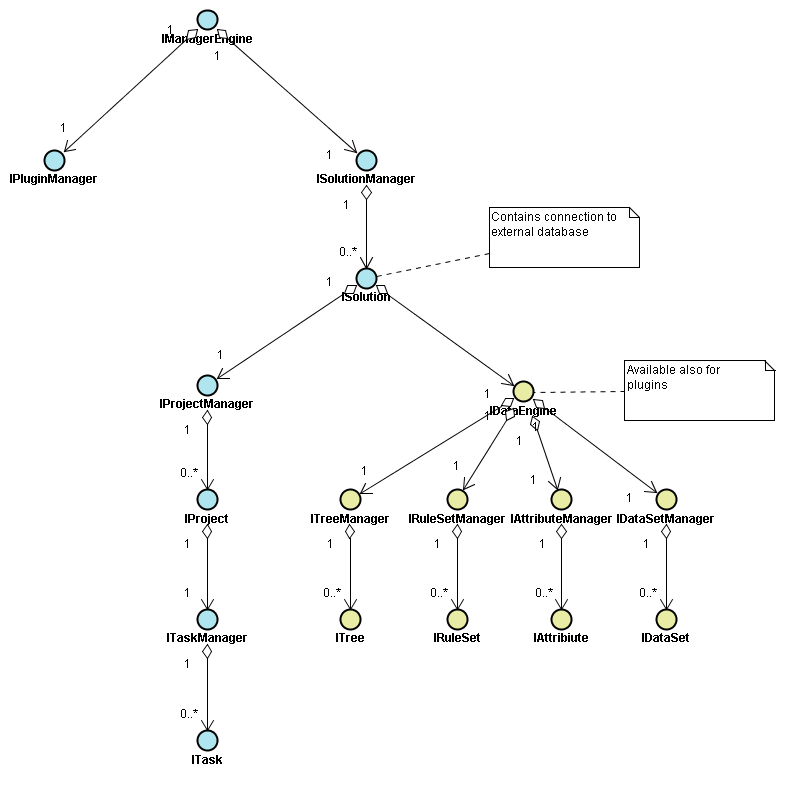
\includegraphics[width=1.00\textwidth]{img/salomon/uml/manager_engine.png}
	\caption{G��wne interfejsy platformy}
	\label{fig:core}
\end{figure}

Interfejsy maj�ce w~nazwie s�owo \emph{Manager} pe�ni� szczeg�ln� funkcj� 
-- najcz�ciej odpowiadaj� za zarz�dzanie innymi interfejsami, np. \emph{IPluginManger} zarz�dza wtyczkami, \emph{IProjectManger} -- projektami.
Dostarczaj� one zestawu metod pozwalaj�cych na wygodne zarz�dzanie obiektami,
ich tworzenie, modyfikowanie, czy usuwanie.
Wszystkie menad�ery maj� analogiczn� funkcjonalno�� -- ka�dy z
nich pozwala na stworzenie nowego obiektu, kt�rym zarz�dza (nie ma innej
mo�liwo�ci ich stworzenia, ni� przez metody udost�pniane przez menad�era), jego
zesk�adowanie w~bazie danych, zwr�cenie wszystkich zarz�dzanych obiekt�w, czy
te� pojedynczego, bazuj�c na unikalnym identyfikatorze oraz usuni�cie konkretnego obiektu.

Menad�ery nie s� dost�pne bezpo�rednio z~platformy, ale
przekazywane s� wtyczkom za pomoc� interfejsu \emph{IDataEngine}.
Wtyczka, zale�nie od potrzeb, pobiera za pomoc� tego interfejsu potrzebny jej menad�er i~za jego
po�rednictwem zarz�dza zbiorem danych, atrybut�w lub drzewem decyzyjnym.

\subsection{IManagerEngine}

Interfejs ten zapewnia dost�p do om�wionych poni�ej menad�er�w.

\paragraph{IPluginManager}

Interfejs \emph{IPluginManager} zarz�dza wtyczkami (por. \ref{lab:plugin}). Pozwala na zapisanie informacji o~nowej wtyczce
(jej nazwie, lokalizacji) oraz na pobranie listy dost�pnych wtyczek.
Mog� one by� �adowane ze zdalnej lokalizacji, a~wi�c zadaniem tego
menad�era jest tak�e zarz�dzanie pobieraniem i~buforowaniem wtyczek pobranych
z zewn�trznych �r�de�.

\paragraph{ISolutionManager}

\emph{ISolutionManager} zarz�dza obiektami implementuj�cymi interfejs \emph{ISolution} (por. \ref{lab:solution}).

\paragraph{IProjectManager}

Interfejs ten umo�liwia zarz�dzanie projektami zdefiniowanymi dla
okre�lonego obiektu \emph{ISolution} (por. \ref{lab:project}) .

\paragraph{ITaskManager}

Interfejs ten dostarcza funkcjonalno�ci umo�liwiaj�cej zarz�dzanie zadaniami (por. \ref{lab:tasks}) dla konkretnego projektu. Opr�cz standardowych operacji wsp�lnych dla wszystkich menad�er�w, jego zadaniem jest tak�e zapewnienie poprawnej konfiguracji, nadz�r nad wykonaniem oraz zachowanie informacji
o przebiegu przetwarzania zada�.

\subsection{IDataEngine}
\label{lab:data_engine}

Obiekt implementuj�cy ten interfejs przekazywany jest wtyczkom podczas ich wykonania.
Za pomoc� pobieranych z~niego menad�er�w jak na przyk�ad \emph{IDataSetManager} 
czy \emph{ITreeManager}
wtyczki mog� operowa� na danych znajduj�cych si� w~bazie.
Udost�pnienie wtyczkom jedynie interfejs�w do operowania na danych pozwala
na ukrycie sposobu sk�adowania danych przed tw�rcami wtyczek i~ich uniezale�nienie si�
od implementacji. W~obecnej wersji dane przechowywane s� w~relacyjnej bazie danych, ale nic nie stoi 
na przeszkodzie, by w~przysz�o�ci przechowywa� je w~inny spos�b, np. w~plikach tekstowych o~ustalonym formacie
czy bazie \emph{LDAP}. Tw�rcy wtyczek nie musz� troszczy� si� o~to, jak dane s� przechowywane, gdy� implementacja
interfejs�w dostarczona jest przez platform�.
Co wi�cej, raz napisane wtyczki b�d� dzia�a� tak�e z~nowszymi jej wersjami,
pod warunkiem zachowania dotychczasowych interfejs�w.

W obecnej wersji wtyczki mog� operowa� na zbiorach danych, atrybutach oraz 
drzewach decyzyjnych odpowiednio za pomoc� interfejs�w \emph{IDataSetManager}, \emph{IAttributeManager} i~\emph{ITreeManager}.
 
\section{Kontrolery}

Kontrolery odpowiadaj� za interakcj�
systemu z~otoczeniem. W~zale�no�ci od konfiguracji systemu przy
starcie uruchamiany jest jeden z~kontroler�w. Kontrolery operuj�
na danych poprzez wsp�lny interfejs, a~co za tym idzie, dane
utworzone poprzez jeden z~nich s� dost�pne pomi�dzy kolejnymi
uruchomieniami programu dla pozosta�ych kontroler�w.

Podstawowym kontrolerem jest \emph{LocalController}. Zarz�dza on zadaniami wykonywanymi na lokalnym komputerze. Zadaniem tego kontrolera jest dostarczenie
interfejsu u�ytkownika, pozwalaj�cego na zarz�dzanie projektami,
wtyczkami i~zadaniami.

Dla potrzeb przetwarzania rozproszonego zdefiniowane zosta�y \emph{MasterController}, kt�rego zadaniem jest zarz�dzanie us�ugami
udost�pnianymi przez zdalne kontrolery (\emph{ServantController}).
Obecna wersja systemu nie uwzgl�dnia tych kontroler�w.

\section{Agenci}
% Poprawic stylistyke
Agenci odpowiadaj� za obs�ug� zdarze� zachodz�cych w~�rodowisku.
W reakcji na zdarzenie wykonuj� odpowiedni� akcj� w~ramach projektu.
Zazwyczaj jest to~przeliczenie ca�ego projektu. Agent mo�e wp�ywa�
na spos�b wykonania projektu, przez odpowiednie ustawienie zmiennych
w �rodowisku (\emph{IEnvironment}).

Agenci mog� reagowa� na r�ne zdarzenia, takie jak na przyk�ad
uaktualnienie informacji w~zewn�trznym �r�dle danych, czy te� pojawienie
si� nowej wiedzy w~wyniku pracy innego agenta. \\
Opr�cz reakcji na zdarzenia
agenci mog� uaktywnia� si� w~okre�lonych odst�pach czasu. 

Interfejsem definiuj�cym agenta jest \emph{IAgent} . Podstawowymi metodami
w nim zawartymi s�:

\begin{itemize}
	\item \emph{void start(IProject project)} -- za pomoc� tej metody uruchamiany jest agent 
		\item \emph{void stop()} -- metoda ta s�u�y do zatrzymania pracy agenta 
		\item \emph{IConfigComponent getConfigComponent();} -- zwraca komponent
pozwalaj�cy u�ytkownikowi na skonfigurowanie agenta

\end{itemize}

\section{Opis bazy danych}

W systemie bardzo wa�n� rol� odgrywaj� baza danych
w kt�rej przechowywane s� ustawienia, projekty, regu�y itp.
Poni�sza struktura dotyczy tylko organizacji danych wykorzystywanych do przetwarzania wiedzy. 
Rzeczywiste dane, na podstawie kt�rych wiedza ta jest tworzona przechowywana 
jest w osobnych bazach danych i dane te nie s� kopiowane do bazy \emph{Salomona}.

\subsection{Struktura platformy}

Dane zosta�y zorganizowane w nast�puj�cych tabelach:

\subsubsection{Solutions}

Tabela reprezentuje obiekty \emph{Solution}, kt�re grupuj� projekty dotycz�ce tej samej tematyki i operuj� na tej samej bazie danych.

\begin{itemize}
		\item \emph{solution\_id} -- identyfikator obiektu \emph{solution}
		\item \emph{solution\_name} -- nazwa		
		\item \emph{solution\_info} -- dodatkowy opis
		\item \emph{hostname} -- host, na kt�rym znajduje si� baza danych
		\item \emph{db\_path} -- �cie�ka do pliku bazy danych na serwerze
		\item \emph{username} -- nazwa u�ytkownika u�ywanego do po��czenia z baz� danych
		\item \emph{passwd} -- has�o potrzebne do zalogowania si�
		\item \emph{lm\_date} -- data ostatniej modyfikacji
\end{itemize}

\subsubsection{Projects}

Tabela zawiera nag��wki projekt�w, do kt�rych odnosz� si� rekordy
z tabeli \emph{Tasks}.

\begin{itemize}
    \item \emph{project\_id} -- identyfikator projektu
    \item \emph{solution\_id} -- powi�zanie z tabel� \emph{solutions}
    \item \emph{project\_name} -- nazwa
    \item \emph{project\_info} -- dodatkowy opis
    \item \emph{env} -- reprezentuje �rodowisko, za pomoc� kt�rego przekazywane s� ustawienia mi�dzy poszczeg�lnymi zadaniami
    \item \emph{lm\_date} -- data ostatniej modyfikacji
\end{itemize}

\subsubsection{Plugins}

Tabela zawiera informacje o pluginach, kt�re mog� by� wykorzystane
przez system. Przechowuje dane o ich nazwach i lokalizacjach, sk�d
mog� by� pobrane.

\begin{itemize}
    \item \emph{plugin\_id} -- identyfikator pluginu
    \item \emph{plugin\_name} -- nazwa pluginu
    \item \emph{plugin\_info} -- dodatkowy opis
    \item \emph{location} -- lokalizacja pluginu
    \item \emph{lm\_date} -- data ostatniej modyfikacji
\end{itemize}

\subsubsection{Tasks}

Tabela zawiera zapis wykonania poszczeg�lnych zada�. Dla ka�dego z nich
przechowywane s� informacje o pluginie, kt�ry zosta�
wykorzystany do wykonania zadania; projekcie, w ramach kt�rego
zadanie zosta�o zapisane; ustawieniach, z jakimi zosta�o wykonane;
rezultacie zadania oraz statusie, w jakim pozostaje po wykonaniu.

\begin{itemize}
    \item \emph{task\_id} -- identyfikator zadania
    \item \emph{task\_nr} -- numer zadania w kolejce do ich wykonania
    \item \emph{project\_id} -- identyfikator projektu, do kt�rego nale�y zadanie
    \item \emph{plugin\_id} -- identyfikator pluginu, kt�ry wykonywany jest w ramach tego zadania
    \item \emph{name} -- nazwa
    \item \emph{info} -- dodatkowy opis
    \item \emph{plugin\_settings} -- ustawienia pocz�tkowe pluginu
    \item \emph{plugin\_result} -- rezultat dzia�ania pluginu
    \item \emph{status} -- status wykonania zadania
\end{itemize}

    Relacje mi�dzy nimi zobrazowane s� na rysunku (Rys \ref{fig:database})

\begin{figure}[H]
	\centering
		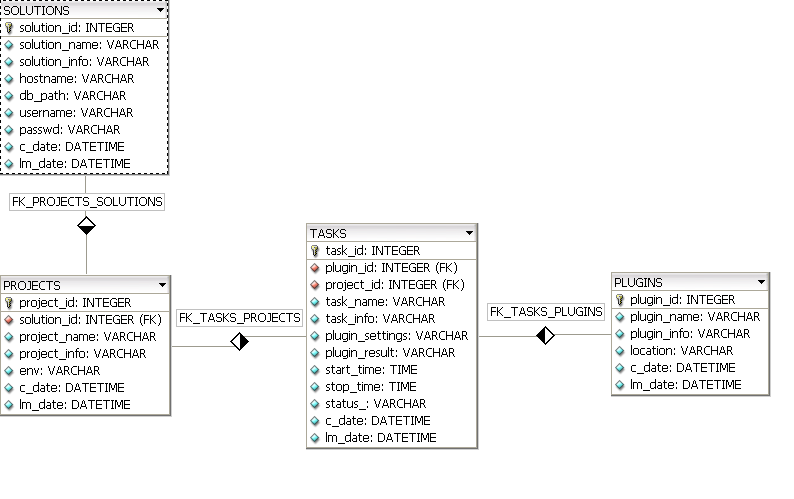
\includegraphics[width=0.90\textwidth]{img/salomon/concept/salomon_db.png}
	\caption{Relacje mi�dzy tabelami platformy}
	\label{fig:database}
\end{figure}

\subsection{Organizacja wiedzy}

\emph{Salomon} wspiera kilka rodzaj�w wiedzy: zbiory danych (\emph{datasets}),
atrybuty oraz drzewa decyzyjne.

\subsubsection{Datasets}

Tabela zawiera nag��wki zbior�w danych.

\begin{itemize}
    \item \emph{dataset\_id} -- identyfikator zbioru danych
    \item \emph{solution\_id} -- powi�zanie z tabel� \emph{solutions}
    \item \emph{dataset\_name} -- nazwa
    \item \emph{dataset\_info} -- dodatkowy opis
    \item \emph{lm\_date} -- data ostatniej modyfikacji
\end{itemize}

\subsubsection{Dataset\_items}

Zawiera definicje zbior�w zada�. Zbi�r danych definiowany jest
przez nazw� tabeli oraz warunki, jakie ograniczaj� rekordy w tej
tabeli. Tabela ta s�u�y do przechowywania podzbioru danych pochodz�cych z rzeczywistej bazy danych.

\begin{itemize}
    \item \emph{dataset\_item\_id} -- identyfikator elementu zbioru danych
    \item \emph{dataset\_id} -- identyfikator zbioru danych, do kt�rego nale�y
element
    \item \emph{table\_name} -- nazwa tabeli
    \item \emph{condition} -- warunek ograniczaj�cy zakres danych
\end{itemize}

\subsubsection{Attributesets}

Tabela zawiera nag��wki zbior�w atrybut�w.

\begin{itemize}
    \item \emph{attributeset\_id} -- identyfikator zbioru atrybut�w
    \item \emph{solution\_id} -- powi�zanie z tabel� \emph{solutions}
    \item \emph{attributeset\_name} -- nazwa
    \item \emph{attributeset\_info} -- dodatkowy opis
    \item \emph{lm\_date} -- data ostatniej modyfikacji
\end{itemize}

\subsubsection{Attributeset\_items}

Tabela przechowuje atrybuty, nale��ce do danego zbioru atrybut�w.
Ka�dy atrybut ma nazw� oraz typ. Obecnie wspierane s� atrybuty typu tekstowego,
numeryczne (ca�kowite i zmiennoprzecinkowe) oraz wyliczeniowe.
Dla atrybut�w typu wyliczeniowego, w polu $attribute_value$ przechowywana jest
lista warto�ci, kt�re dany atrybut mo�e przyjmowa�.
Atrybuty odpowiadaj� kolumnom z bazy danych, st�d ka�dy z nich przechowuje
odwolanie do kolumny w tabeli, na podstawie kt�rej zosta� zdefiniowany. 

\begin{itemize}
  	\item \emph{attributeset\_item\_id} -- identyfikator atrybutu
    \item \emph{attributeset\_id} -- identyfikator zbioru atrybut�w, do kt�rego
    dany atrybut nale�y
    \item \emph{solution\_id} -- powi�zanie z tabel� \emph{solutions}
    \item \emph{attribute\_name} -- nazwa
    \item \emph{attribute\_type} -- typ atrybutu
	\item \emph{table\_name} -- nazwa tabeli, na podstawie kt�rej atrybut zosta�
	zdefiniowany
	\item  \emph{column\_name} -- nazwa kolumny z tej tabeli
	\item  \emph{attribute\_value} -- lista warto�ci, kt�re atrybut mo�e
	przyjmowa�. Dotyczy atrybut�w typu wyliczeniowego.
\end{itemize}

\subsubsection{Trees}

Tabela przechowuje nag��wki drzew decyzyjnych. Zawiera odniesienie do zbioru
atrybut�w, gdy� to w�a�nie na ich podstawie drzewa s� budowane.

\begin{itemize}
  	\item \emph{tree\_id} -- identyfikator drzewa decyzyjnego
    \item \emph{attributeset\_id} -- identyfikator zbioru atrybut�w
    \item \emph{solution\_id} -- powi�zanie z tabel� \emph{solutions}
    \item \emph{root\_node\_id} -- identyfikator korzenia drzewa
    \item \emph{tree\_name} -- nazwa
    \item \emph{tree\_info} -- dodatkowy opis
    \item \emph{lm\_date} -- data ostatniej modyfikacji
\end{itemize}

\subsubsection{Tree\_nodes}

Zawiera definicje w�z��w drzewa decyzyjnego.

\begin{itemize}
  	\item \emph{node\_id} -- identyfikator w�z�a
  	\item \emph{tree\_id} -- identyfikator drzewa decyzyjnego, do kt�rego nale�y
    \item \emph{parent\_node\_id} -- identyfikator w�z�a rodzica (0 dla korzenia)
    \item \emph{attribute\_item\_id} -- identyfikator atrybutu, kt�remu w�ze� odpowiada
    \item \emph{parent\_edge\_value} -- warunek na kraw�dzi prowadz�cej do w�z�a
    \item \emph{node\_value} -- warto�� w w�le
\end{itemize}





\section{Wtyczki}

System, dzi�ki swej elastycznej architekturze, pozwala u�ytkownikowi na 
rozszerzanie jego mo�liwo�ci poprzez definiowanie przez niego w�asnych 
wtyczek. Dzi�ki takiemu podej�ciu system jest �atwo skalowalny
i rozszerzalny o~nowe mo�liwo�ci. 

Ca�a funkcjonalno�� zwi�zana z~konfiguracj�  przetwarzaniem, prezentacj� wynik�w dzia�ania oraz komunikacj� przez sie� ukryta jest przed tw�rc� wtyczki i~nie musi by� brana pod uwag� przy jego projektowaniu i~implementacji. Jedyne, co musi on zrobi� to~zaimplementowa� opisane poni�ej interfejsy.
By system m�g� skorzysta� z~nowych wtyczek nale�y 
poda� ich lokalizacje, umo�liwiaj�c systemowi tym samym pobranie i~
za�adowanie wtyczki. Obecna wersja systemu obs�uguje tylko wtyczki w~postaci 
archiw�w jar.

Poni�y diagram (Rys. \ref{fig:plugin_uml}) przedstawia podstawowe interfejsy
potrzebne do implementacji w�asnej wtyczki. Kolorem ��tym zaznaczone
zosta�y interfejsy zwi�zane z~graficzn� cz�ci� wtyczki. Kolorem niebieskim
interfejs, kt�ry zwi�zany jest z~algorytmem wtyczki. 

\begin{figure}[H]
	\centering
		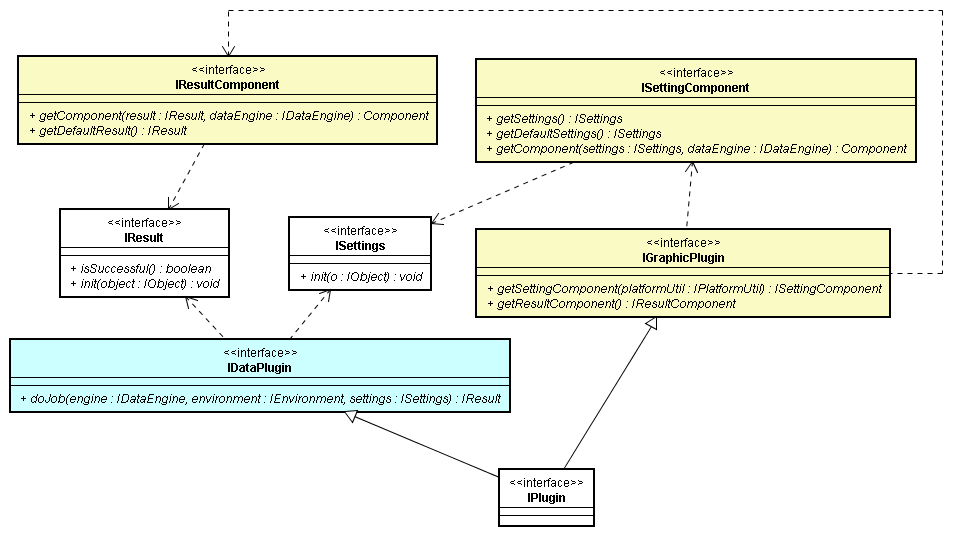
\includegraphics[width=0.90\textwidth]{img/salomon/uml/plugin.png}
	\caption{Interfejsy wtyczki}
	\label{fig:plugin_uml}
\end{figure}

\subsection{IPlugin}

Jest to~g��wny interfejs implementowany przez wszystkie wtyczki. Stanowi po��czenie interfejs�w \emph{IDataPlugin}~(\ref{lab:data_plugin}) i~\emph{IGraphicPlugin}~(\ref{lab:graphic_plugin}).
 
\subsection{IDataPlugin}
\label{lab:data_plugin}

Interfejs ten definiuje tylko jedn� metod� \emph{doJob()}, kt�ra jest uruchamiana podczas przetwarzania danej wtyczki i~stanowi jej g��wne zadanie obliczeniowe. Jej parametry to:

\begin{itemize}
	\item \emph{IDataEngin}~(\ref{lab:data_engine}) -- obiekt ten dostarcza interfejs�w pozwalaj�cych na operowanie na danych i~wiedzy (np. ITreeManager)
 	\item \emph{IEnvironment} to~interfejs umo�liwiaj�cy komunikacje 
          pomi�dzy poszczeg�lnymi zadaniami
	\item \emph{ISettings} reprezentuj� konfiguracja wej�ciowa wtyczki
\end{itemize}  
    
\subsection{IGraphicPlugin}
\label{lab:graphic_plugin}
Interfejs ten okre�la spos�b, w~jaki wtyczka mo�e by� konfigurowana przez u�ytkownika oraz jak maj� by� prezentowane wyniki oblicze�. 
\begin{itemize}
	\item \emph{getSettingComponent()} -- zwraca obiekt implementuj�cy interfejs 
		\emph{ISettingComponent}~(\ref{lab:setting_component})
	\item \emph{getResultComponent()} -- zwraca obiekt implementuj�cy interfejs 
		\emph{IResultComponent}~(\ref{lab:result_component})
\end{itemize}

\subsection{ISettingComponent}
\label{lab:setting_component}
\begin{itemize}
	\item \emph{getComponent(ISettings settings)} -- zwraca graficzny komponent 
s�u��cy do edycji ustawie� wtyczki. Jest on wype�niany warto�ciami przekazanymi 
w obiekcie \emph{ISettings}.
	\item \emph{getSettings()} -- zwraca ustawienia wtyczki.
	\item \emph{getDefaultSettings()} -- zwraca domy�lne ustawienia wtyczki. 
Wykorzystywane, gdy u�ytkownik nie wprowadzi� w�asnych ustawie�.
\end{itemize}    

\subsection{IResultComponent}
\label{lab:result_component}
\begin{itemize}
	\item \emph{getComponent(IResult result)} -- zwraca graficzny komponent 
wy�wietlaj�cy rezultat wykonania wtyczki. Wype�niany jest on na podstawie 
obiektu  \emph{IResult} zwr�conego wcze�niej przez metod� \emph{doJob()}.
	\item  \emph{getDefaultResult()} -- zwraca domy�lny rezultat wykonania wtyczki.
\end{itemize}

\subsection{IObject} To~interfejs zapewniaj�cy persystencj� takich obiekt�w 
jak ustawienia, rezultat wykonania wtyczki, czy obiekty wykorzystywane do komunikacji mi�dzy wtyczkami.

\subsection{ISettings}Implementowany przez obiekt reprezentuj�cy ustawienia 
wtyczki.
\begin{itemize}
	\item \emph{init(IObject o)} - metoda inicjalizuje obiekt klasy
\end{itemize}    

\subsection{IResult} Implementowany przez obiekt reprezentuj�cy rezultat 
dzia�ania wtyczki.
\begin{itemize}
	\item \emph{init(IObject o)} - metoda inicjalizuje obiekt klasy
\end{itemize}  

%WSTAWI� TO W~JAKIE� MIEJSCE!!!
%
%\paragraph{Persystencja danych}
%Z racji na rozproszony charakter aplikacji, oraz na wielko�� oblicze�.
%Wa�nym aspektem platformy jest zapewnienie uniwersalnego i~wydajnego
%mechanizmu persyste�cji danych. W~przypadku wewn�trznych struktur danych,
%jak zapis drzewa decyzyjnego, czy atrybut�w, zadaniem tym zajmuj� si�
%odpowiednie menadz�ry. W~przypadku jednak persystencji danych u�ytkownika,
%takich jak ustawienia wtyczek, czy ich rezultaty zadaniem tym zajmuj� si�
%modu� persyste�cji, udost�pniaj�cy odpowiedni \emph{API}. Dodatkowo mechanizm
%ten jest wykorzystywany do persystencji danych wykorzystywanych w~komunikacji mi�dzy kolejnymi zadaniami (WSTAWI� LINKA DO OPISU ENV.)
%
%Kod poni�ej tworzy struktur�, z~jednym polem o~nazwie ,,myField'' oraz przypisuje do niego warto�� ,,my settings''.
%
%\begin{lstlisting}
%SimpleStruct struct = new SimpleStruct();
%struct.setField("myField", "my settings");
%\end{lstlisting}
%
%WSTAWI� UML? 



\section{Uruchomienie}
Do uruchomienia programu konieczne jest zainstalowanie w systemie \emph{Java Runtime Environment} , w wersji 1.5. Je�li program ma dzia�a� z wykorzystaniem niezale�nego serwera bazy danych \emph{Firebird}, to nale�y zainstalowa� dodatkowo baz� \emph{Firebird}.

Program mo�e dzia�a� w 3 trybach (jako serwer, klient lub lokalnie) i na dwa sposoby ��czy� si� z baz� danych (poprzez serwer lub bez niego), zale�nie od wpis�w w pliku konfiguracyjnym. 
Aby uruchomi� go w odpowiedniej konfiguracji, nale�y rozpakowa� go i zmodyfikowa� domy�lne ustawienia pliku konfiguracyjnego. Program dostarczany jest z przyk�adow� baz� danych w kt�rej zdefiniowane s� odpowiednie tabele i lokalizacje plugin�w oraz z przyk�adowymi pluginami. 
Dla u�ytkownik�w, kt�rzy chc� stworzy� w�asn� baz� danych w katalogu db umieszczony zosta� skrypt, tworz�cy tabele niezb�dne do pracy programu i uruchomienia dostarczonych plugin�w (crebas.sql).

\subsection{Plik konfiguracyjny}
G��wnym plikiem konfiguracyjnym programu jest config.properties.
Zawiera on nast�puj�ce klucze:

\begin{itemize}
\item \emph{HOSTNAME} - identyfikator sieciowy komputera, na kt�rym zainstalowana jest baza danych. Uwzgl�dniany jest tylko w przypadku, gdy program ��czy si� z baz� danych przy u�yciu serwera Firebird.

\item \emph{DB\_PATH} - lokalizacja bazy danych. Gdy program dzia�a z serwerem Firebird jest to lokalizacja bezwzgl�dna, w przeciwnym przypadku - wzgl�dem katalogu instalacyjnego.

\item \emph{USER} - nazwa u�ytkownika, kt�ry loguje si� do bazy

\item \emph{PASSWD} - has�o u�ytkownika

\item \emph{EMBEDDED} - okre�la, spos�b po��czenia z baz� danych
\subitem \emph{N} - z wykorzystaniem serwera
\subitem \emph{Y} - przy u�yciu dll-a

\item \emph{SERVER\_HOST} - nazwa komputera, na kt�rym zainstalowany jest Salomon w wersji server

\item \emph{SERVER\_PORT} - port na kt�rym nas�uchuje server

\item \emph{MODE - tryb} uruchomienia
\subitem \emph{local} - lokalnie
\subitem \emph{client} - klient
\subitem \emph{server} - serwer

\end{itemize}

Pozosta�e warto�ci nie powinny by� modyfikowane przez u�ytkownika.

\subsection{Ustawienia pliku konfiguracyjnego}
\paragraph{Tryb serwera}
\begin{itemize}
    \item \emph{MODE=server}
    \item \emph{SERVER\_HOST=IP hosta}
    \item \emph{SERVER\_PORT=nr portu}
\end{itemize}

\paragraph{Tryb klienta}
\begin{itemize}
    \item \emph{MODE=server}
    \item \emph{SERVER\_HOST=IP sewera}
    \item \emph{SERVER\_PORT=nr portu na kt�rym nas�uchuje serwer}
\end{itemize}

\paragraph{Tryb lokalny}
\begin{itemize}
    \item \emph{MODE=local}
\end{itemize}

We wszystkich trybach mo�liwe jest ustawienie po��czenie z baz� danych za pomoc� serwera Firebird lub przy u�yciu dll-a (klucz \emph{EMBEDDED}).

\section{Interfejs u�ytkownika}

\subsection{Tryb serwera}
G��wnym zadaniem systemu jest umo�liwienie definiowania i wykonywania zada� w oparciu o dost�pne pluginy. Gdy program dzia�a w trybie serwera po lewej stronie widoczna jest lista pod��czonych klient�w. Wszystkie opisane poni�ej operacje wykonywane s� dla aktualnie wybranego klienta.

\subsubsection{Zadania}
Aby zdefiniowa� nowe zadanie, nale�y wybra� plugin, za pomoc� kt�rego b�dzie ono realizowane oraz skonfigurowa� jego ustawienia. Plugin nale�y wybra� z listy dost�pnych plugin�w, znajduj�cej si� na �rodku g��wnego okna programu. Po wybraniu pluginu i naci�ni�ciu przycisku ze strza�k� w prawo znajduj�cego si� miedzy panelem z pluginami a panelem z zadaniami pojawia si� okienko, w kt�rym nale�y wprowadzi� nazw� zadania. 


%\paragraph{@@@PIPCZER}
\paragraph{}

Po potwierdzeniu nazwy zostanie utworzone nowe zadanie i dodane do listy zada�. Ka�de z zada� mo�na skonfigurowa� przed wykonaniem, w tym celu nale�y nad wybranym zadaniem wywo�a� menu kontekstowe (prawym klawiszem myszy) i wybra� opcj� \textbf{Settings}. Po jej wybraniu pojawi si� okienko s�u��ce do konfiguracji zadania - mo�e by� r�ne, zale�nie od pluginu kt�ry ma by� wykonany w ramach zadania. 

%\paragraph{@@@PIPCZER}


\paragraph{}
Po skonfigurowaniu zada� nale�y zatwierdzi� list� zada� do wykonania za pomoc� klawisza \textbf{Apply}. Je�li zadania nie zosta�y wcze�niej zapisane w ramach projektu, pojawi si� okienko w kt�rym nale�y poda� nazw� projektu. Po poprawnym zapisaniu projektu mo�na wykona� zaplanowane zadania. Zostan� one wykonane  w takiej kolejno�ci, w jakiej znajduj� si� one na li�cie zada�. Mo�liwa jest zmiana tej kolejno�ci - s�u�� do tego przyciski ze strza�kami znajduj�ce si� po prawej stronie panelu z zadaniami. Je�li zostanie ustalona ostateczna kolejno�� zada�, mo�na je wykona� za pomoc� przycisku Run.

\paragraph{}
Po wykonaniu zada� mo�na obejrze� ich rezultaty. W tym celu nale�y z menu kontekstowego dla zada� wybra� opcj� \textbf{Result}. Po jej wybraniu pojawi si� okienko prezentuj�ce wyniki wykonania danego zadania. Jego wygl�d, podobnie jak w przypadku ustawie� zada�, zale�y od pluginu.

\subsubsection{Pluginy}
Lista plugin�w tworzona jest na podstawie odpowiednich wpis�w w bazie danych. Mo�na j� jednak  modyfikowa� - dodawa�, usuwa� lub modyfikowa� dane pluginy. S�u�� do tego odpowiednie opcje z menu kontekstowego wywo�ywanego dla plugin�w. 

%\paragraph{@@@PIPCZER}


\subsubsection{Projekty}

Konfiguracja plugin�w oraz lista zada� zapisywana jest w ramach projekt�w. Dzi�ki temu mo�na zdefiniowa� r�ne listy zada� i wykonywa� je wielokrotnie, bez potrzeby ich ponownego tworzenia i konfiguracji. Aby za��dowa� istniej�cy projekt nale�y z menu g��wnego wybra� pozycj� \textbf{Projects$\rightarrow$Open Project}. Spowoduje to wy�wietlenie listy zapisanych projekt�w i umo�liwi wyb�r projektu do za�adowania. 

\subsection{Tryb klienta}
Program pracuj�cy w tym trybie nie posiada interfejsu u�ytkownika, jego konfiguracja odbywa si� z serwera.

\subsection{Tryb lokalny}
Interfejs dla programu dzia�aj�cego w trybie lokalnym zbli�ony jest do programu w trybie serwera. Nie posiada on jednak listy pod��czonych klient�w, gdy� sam wykonuje zdefiniowane zadania, czyli zachowuje si� jak po��czenie dw�ch program�w dzia�aj�cych w trybie serwera i klienta.

\subsection{SQL Console}
W trybie serwera oraz w trybie lokalnym z menu Tools dost�pny jest program SQL Console. Pozwala on na wykonywanie zapyta� SQL-owych, przez co umo�liwia administracj� projektami, pluginami i zadaniami oraz innymi tabelami wykorzystywanymi przez system.


\section{Za�o�enie implementacyjne}
W czasie produkcji systemu stosowali�my nast�puj�ce zasady:

\subsection{Kontrola wersji}
Ca�y kod oraz inne zasoby wykorzystywane w programie znajduj� si� pod kontrol� wersji. U�ywany do tego jest  \emph{Subversion} (nast�pca CVS-a) i odpowiednie pluginy zapewniaj�ce jego integracj� z edytorem oraz systemem operacyjnym. Zapewnia to pe�n� synchronizacj� kodu na wszystkich komputerach, na kt�rych mo�e on by� modyfikowany.

\subsection{Wsp�lny edytor}
U�ywany jest wsp�lny edytor - \emph{Eclipse}. Dzi�ki mo�liwo�ci eksportowania ustawie� u�ywane jest  identyczne formatowanie kodu, co pomaga utrzyma� przejrzysto�� i czytelno�� kodu. 

\subsection{Testowanie jednostkowe} 
W celu testowania funkcjonalno�ci wykorzystujemy mechanizm \emph{JUnit}. 

\subsection{GUI testowanie}
W celu weryfikowania poprawno�ci interfejsu u�ytkownika stworzone zosta�y skrypty dla programu Abbot. Jego zadaniem jest odtworzenie nagranych sekwencji wykonywanych  przez  u�ytkownika w czasie obs�ugi programu. W po��czeniu z runtime-ow� weryfikacj� kontrakt�w stanowi to silny mechanizm weryfikacji jako�ci produktu

\subsection{Kontrakty}
W kodzie zosta�y wprowadzone mechanizmy zaczerpni�te z j�zyka  \emph{Eiffel} - tzw. kontrakty. Polega to na tym, �e w komentarzach dla klas oraz metod zawarte s� warunki, sprawdzaj�ce poprawno�� stanu, w jakim znajduje si� system. Kontrakty stanowi� dodatkow� informacj� dla programisty wykorzystuj�cego dan� klas� lub interfejs. Dodatkowo wykorzystywany jest kompilator, kt�ry kompiluje tak�e kod kontrakt�w i w razie ich z�amania rzuca wyj�tki.

\subsection{Automatyczne budowanie projektu} 
W celu zautomatyzowania procesu budowania projektu wykorzystany zosta� program  \emph{Ant}. Automatyzuje on proces tworzenia projektu od kompilacji, a� do wygenerowania instalatora.

\subsection{Instalator}
By upro�ci� proces instalacji dla u�ytkownika ko�cowego utworzone zosta�y skrypty tworz�ce instalator. Jako program do utworzenia instalatora wykorzystywany jest program  \emph{IzPack}.

\subsection{Mechanizmy lokalizacyjne}
Wszystkie teksty u�yte w interfejsie u�ytkownika pobierane s� z odpowiednich plik�w, co pozwala na �atw� lokalizacj� programu

\subsection{Konfiguracja}
Konfiguracja programu wczytywana jest z odpowiednich plik�w konfiguracyjnych. Pozwala to na �atw� zmian� zachowania programu (np. zmian� kontrolera). 

\subsection{Logowanie}
Do �ledzenia przebiegu wykonania programu wykorzystywany jest log4j. Wprowadza on elastyczny model logowania. 

\subsection{Zarz�dzanie projektem}
Jak system zarz�dzania projektem wybrali�my Gemini - system wspomagania pracy grupowej oparty na ASP.NET. System wspomaga wszelkie dziedziny �ycia projektu, poczynaj�c od przydzia�u zada� dla poszczeg�lnych developer�w, kontroli stanu ich wykonania, estymacji czasu pracy nad danym zagadnieniem, po zarz�dzanie projektem jak ca�o�ci� czyli wyznaczanie milestone'�w oraz przypisywania do nich zada�, generacja diagram�w Gantta, zarz�dzanie zasobami ludzkimi itp. 

%\subsection{CMS}
%Jako CMS(Content Management System) dla naszej strony zosta� u�yty projekt Mambo 4.9.1a. Jest to bardzo wygodny i %elastyczny w u�ytkowaniu system kontroli tre�ci. System ma budow� modu�ow� dzi�ki czemu mo�emy w ka�dej chwili rozszerzy� %jego funkcjonalo��. Opr�cz standardowych modu��w jakie dostarczane s� z dystrybucj� Mambo do��czyli�my Forum dyskusyjne %(SimpleBoard) oraz galeri� (RSGallery). Dodatkow� mo�liwo�ci� jest wrappowanie innych projekt�w dzi�ki czemu uda�o nam %sie bez wi�kszych problem�w doda� modu�y bezpo�rednio nie wspierane przez Mambo, jak Bugzilla czy Wiki.


%\subsection{Maven}
%W projekcie u�yli�my r�wnie� mavena. Jest to bardzo u�yteczne narz�dzie do zarz�dzania buildami, jak r�wnie� tworzeniem raport�w na temat posuwaj�cych si� prac. Aktualnie podpi�li�my nast�puj�ce raporty:
%\begin{itemize}
%	\item Changes\\
%	w estetyczny spos�b pokazuje wersje, i zmiany jakie w nich zasz�y
%	\item Checkstyle\\
%	raport z checkstyle'a \href{http://checkstyle.sourceforge.net/}{http://checkstyle.sourceforge.net/}, najpopularniejszego chyba darmowego narz�dzia do statycznej analizy kodu)
%	\item Unit tests\\
%	Raport z przebiegu test�w wykonanych za pomoc� JUnita
%	\item File activity\\
%	Pokazuje jak cz�sto zmienia�y si� poszczeg�lne pliki
%	\item Change log\\
%	Pokazuje komentarze z wszystkich commit�w do repozytorium
%	\item PMD report\\
%	to narz�dzie(\href{http://pmd.sourceforge.net/}{http://pmd.sourceforge.net/}) wykrywa potencjalne b��dy, takie jak:
	
%		\begin{itemize}
%			\item puste bloki try/catch/finally/switch
%			\item nieu�ywane lokalne zmienne, parametry i metody prywatne
%			\item puste warunki: if/while
%		\end{itemize}
%	\item Javadocs
%	\item Kod w postaci plik�w html
%\end{itemize}

\section{Wtyczki}

\subsection{Tworzenie zbioru danych}

By u�atwi� generowanie testowych zbior�w danych utworzone zosta�y 2 wtyczki:
\emph{DataSetCreator} i \emph{RandomDataSetCreator}.

Zadaniem obydwu z nich jest utworzenie zbioru danych o podanej przez u�ytkownika
nazwie i zapisanie jego struktury w bazie danych. Jako, �e wtyczki nie maj�
bezpo�redniego dost�pu do g��wnej bazy danych \emph{Salomona}, do tworzenia
i~zapisywania zbior�w danych wykorzystuj� menad�era zbior�w danych
(\emph{IDataSetManager}).

Ich dzia�anie jest zbli�one, r�ni� si� tylko rodzajem danych wej�ciowych.
\emph{DataSetCreator} pozwala u�ytkownikowi na dok�adne wyspecyfikowanie jakie
warunki musz� spe�nia� poszczeg�lne rekordy, np. bazuj�c na relacji Osoby, 
w wynikowym zbiorze danych mog� si� znale�� tylko takie, kt�rych wiek przekracza
20 lat, a nazwisko zaczyna  si� na liter� ,,K''. 

Wykorzystanie tej wtyczki pozwala na dok�adne okre�lenie
interesuj�cego zbioru danych, jednak jest dosy� pracoch�onne.
W przypadku, gdy nie jest wa�ne, kt�re konkretnie rekordy znajd� si� w wynikowym
zbiorze danych lepiej pos�u�y� si� wtyczk� \emph{RandomDataSetCreator}. 
Podobnie jak wtyczka \emph{DataSetCreator} pozwala ona na okre�lenie, kt�re
kolumny z poszczeg�lnych relacji maj� by� uwzgl�dniane w wynikowym zbiorze
danych, jednak poszczeg�lne wiersze dobierane s� losowo. U�ytkownik okre�la
tylko, ile wierszy z danej relacji ma znale�� si� w wygenerowanym zbiorze danych.

Obie wtyczki oferuj� podobny graficzny interfejs u�ytkownika. Panel z
ustawieniami wtyczki pozwala na wyb�r kolumn z poszczeg�lnych relacji, kt�re
maj� znale�� si� w wygenerowanym zbiorze danych. W przypadku wtyczki
\emph{DataSetCreator} dodatkowo okre�la si�, jakie waruneki maj� spe�ania�
rekordy (Rys \ref{fig:datasetcreator}), 
a wtyczka \emph{RandomDataSetCreator} wymaga podania ilo�ci
wiersz�w z poszczeg�lnych relacji, kt�re maj� by� wygenerowane.

\begin{figure}[H]
	\centering
		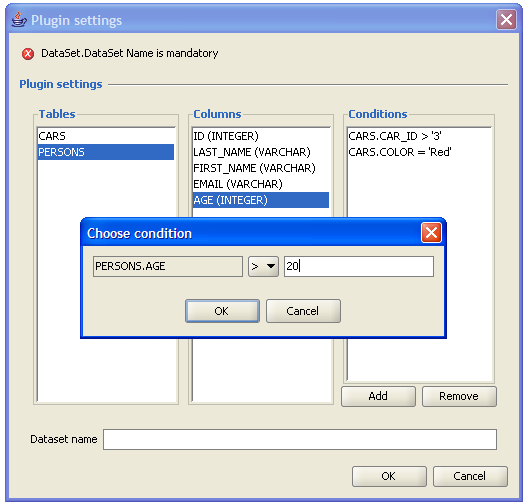
\includegraphics[width=0.90\textwidth]{img/salomon/plugins/datasetcreator.png}
	\caption{Wprowadzanie ustawie� wtyczki DataSetCreator}
	\label{fig:datasetcreator}
\end{figure}

\subsection{Tworzenie zbioru atrybut�w}

Tworzenie zbioru atrybut�w odbywa si� za pomoc� wtyczki
\emph{AttributeSetCreator}.  

Jej zadaniem jest utworzenie zbioru atrybut�w, kt�ry mo�e potem zosta�
wykorzystany np. do budowy drzewa decyzyjnego.

Ka�dy atrybut odpowiada kolumnie relacji z bazy danych, posiada tak�e dodatkowo
typ oraz w�a�ciwo�� okre�laj�c�, czy jest to atrybut decyzyjny. 

Graficzny interfejs s�u��cy do tworzenia zbioru atrybut�w jest podobny do
interfejsu wtyczek tworz�cych zbiory danych. Pozwala na wyb�r kolumny, kt�rej
nowy atrybut ma odpowiada�, wprowadzenie nazwy atrybutu, okre�lenie jego typu
(liczba ca�kowita, liczba zmiennoprzecinkowa, tekstowy i wyliczeniowy) oraz
tego, czy jest to atrybut decyzyjny (Rys \ref{fig:attrsetcreator}). 

\begin{figure}[H]
	\centering
		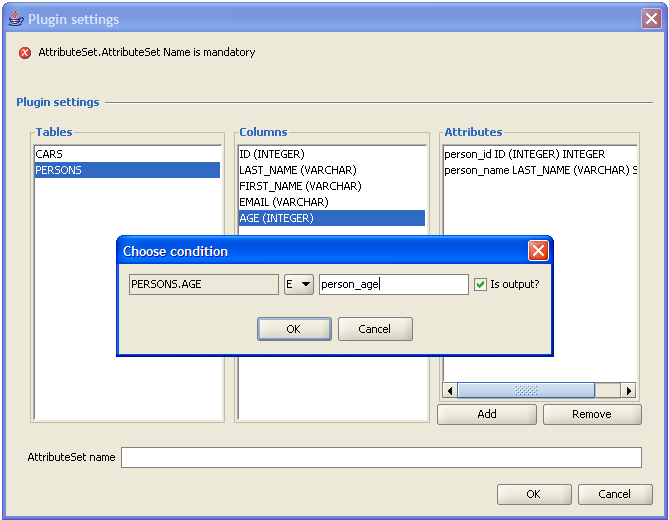
\includegraphics[width=0.90\textwidth]{img/salomon/plugins/attrsetcreator.png}
	\caption{Wprowadzanie ustawie� wtyczki AttributeSetCreator}
	\label{fig:attrsetcreator}
\end{figure}

W danym zbiorze danych musi znajdowa� si� dok�adnie jeden atrybut decyzyjny.
W przypadku atrybut�w wyliczeniowych przyj�to za�o�enie, �e warto�ci, kt�re mo�e
on przyjmowa� to te, kt�re przechowuje kolumna w relacji, kt�rej odpowiada.




\chapter{Eksperyment}

%%
\mgrclosechapter
%%
%% ==== ROZDZIA� 2 ====
%%
%\input{Mgr_roz2}
%%
%%
%% ======== DODATKI ========
%%
%%
%% ======== BIBLIOGRAFIA ========
%%
\newpage

\begin{thebibliography}{99}
\bibitem {bib2} {Kaufman, K. and Michalski, R.S., The Development
    of the Inductive Database System VINLEN: A Review of Current
    Research, International Intelligent Information Processing and
    Web Mining Conference, Zakopane, Poland, 2003}

\bibitem {bib3} {Michalski, R.S. and Kaufman, K., Data Mining and
    Knowledge Discovery: A Review of Issues and a Multistrategy
    Approach, Machine Learning and Data Mining: Methods and
    Applications, R. S. Michalski, I. Bratko and M.  Kubat (Eds.), pp.
    71-112, London: John Wiley \& Sons, 1998}

\bibitem {bib4} {Michalski, R.S., Knowledge Mining and Inductive
    Databases: An Emerging New Research Direction, School of
    Computational Sciences, George Mason University, 2004}

\bibitem {yale} {Mierswa, I., Klinkenberg, R., Fischer, S., Ritthoff, O.,
    A Flexible Platform for Knowledge Discovery Experiments:
    YALE -- Yet Another Learning Environment,
    LLWA 03 - Tagungsband der GI-Workshop-Woche Lernen - Lehren - Wissen -
    Adaptivit�t, 2003.}

\bibitem{uci} {Newman, D.J., Hettich, S., Blake, C.L., Merz, C.J.,
UCI Repository of machine learning databases, Irvine, CA, 1998.}

\bibitem {weka} {Witten, I.H., Frank, E., Data Mining: Practical Machine Learning Tools and
Techniques, Morgan Kaufmann, 2005}



\end{thebibliography}

%%
%% ======== DODATKOWE ELEMENTY PRACY (nieobowi�zkowe) ======== 
%%
\printindex  
%%

\end{document}